\documentclass[letterpaper,journal]{IEEEtran}

\usepackage{amsmath,amssymb}
\usepackage{fontspec}
\usepackage{xeCJK}
\setmainfont{TeX Gyre Termes}
\setsansfont{TeX Gyre Heros}
\setmonofont{Latin Modern Mono}
\setCJKmainfont{FandolSong-Regular}[
    BoldFont=FandolSong-Bold,
    ItalicFont=FandolFang-Regular,
    BoldItalicFont=FandolHei-Bold
]
\setCJKsansfont{FandolHei-Regular}[BoldFont=FandolHei-Bold]
\setCJKmonofont{FandolFang-Regular}
\XeTeXlinebreaklocale "zh"
\XeTeXlinebreakskip=0pt plus 1pt

\usepackage{algorithm}
\usepackage{algorithmic}
\usepackage{array}
\usepackage{booktabs}
\usepackage{cite}
\usepackage{graphicx}
\usepackage{placeins}
\usepackage{url}
\usepackage{xcolor}
\usepackage{tikz}
\usetikzlibrary{arrows.meta,positioning}

\graphicspath{{paper_assets/}}
\newcolumntype{L}[1]{>{\raggedright\arraybackslash}p{#1}}
\renewcommand{\abstractname}{摘要}
\renewcommand{\IEEEkeywordsname}{关键词}
\renewcommand{\figurename}{图}
\renewcommand{\tablename}{表}
\renewcommand{\refname}{参考文献}
\floatname{algorithm}{算法}

\hyphenation{RMTGP ACOTSP phero-mone}

\begin{document}

\title{基于残差多树遗传编程的蚁群优化状态转移与信息素更新规则联合设计}

\author{第一作者，第二作者，第三作者%
\thanks{作者姓名、单位和基金信息将在内部评审后补充。}}

\markboth{IEEE Transactions 中文草稿，2026年8月}%
{作者等：面向蚁群优化的残差多树遗传编程}

\maketitle

\begin{abstract}
蚁群优化的性能主要取决于状态转移规则和信息素更新规则。
这两类规则通常由研究者手工设计。
遗传编程可以自动生成规则。
但是，直接替换完整规则可能破坏原算法中有效的结构。
本文提出残差多树遗传编程蚁群优化方法，简称 RMTGP-ACO。
该方法使用两棵强类型树。
第一棵树对状态转移分数进行有界修正。
第二棵树在固定预算内重新分配信息素增量。
当两棵树都输出零时，算法严格退化为原始 ACO。
本文在 AS、ACS 和 MMAS 上实现该方法。
第一组实验不使用局部搜索，并只在均匀 TSP100 上训练。
Full-F1 在 12 个“算法变体--规模”组合中均降低了平均参考差距。
它还在六个匹配的 TSP100/TSP500 对比中优于重新训练的上一篇研究表示。
控制消融表明，残差方式并不总是优于完整替换。
双树、Full 终端集和 F1 函数集也没有稳定的普遍优势。
随后，本文分析 2-opt 对 GP 学习信号的影响。
在 TSP100 信号审计中，2-opt 后的程序间最终差距方差仅为搜索前的
1.08--3.47\%。
为此，本文引入局部搜索感知终端、多保真适应度和三阶段 TSP500 训练。
在均匀、聚类和高斯 TSP500 上，AS 模型相对 ACO+2-opt 分别降低
55.8\%、32.1\% 和 50.0\% 的差距。
它在均匀集和高斯集上优于 ACO+3-opt，但在聚类集上没有达到该结果。
ACS 和 MMAS 没有得到同样的收益。
融合 CUDA 评估器在登记的基准上取得了相对 16 线程 CPU 的
14.626 倍单 GPU 加速。
所有进化条件均使用三个独立 GP 运行，因此结果按先导证据解释。
\end{abstract}

\begin{IEEEkeywords}
蚁群优化，遗传编程，超启发式，多树遗传编程，残差学习，旅行商问题。
\end{IEEEkeywords}

\section{引言与研究动机}

蚁群优化（ant colony optimization, ACO）通过信息素和启发式信息构造解
\cite{dorigo1996antsystem,dorigo2004aco}。
状态转移规则决定下一步选择。
信息素更新规则决定后续搜索分布。
这两类规则都很重要。
现有算法通常使用固定公式。

遗传编程（genetic programming, GP）可以进化可执行表达式
\cite{koza1992gp,poli2008fieldguide}。
上一篇 GP-ACO 工作直接进化完整的状态转移规则 \cite{lin2025gpaco}。
该方法证明了自动设计规则的可行性。
但是，完整替换会删除原 ACO 的分数结构。
进化表达式也可能产生过大的数值。
此外，状态转移和信息素更新之间存在反馈关系。
只学习其中一个部分可能限制搜索能力。

本文研究一个简单问题：能否保留原 ACO 的主体，只让 GP 学习有限的修正？
为此，本文提出 RMTGP-ACO。
方法包含一棵状态转移树和一棵信息素树。
两棵树使用不同的强类型。
它们共享同一个适应度和同一个总节点预算。

本文的技术贡献如下。
\begin{itemize}
    \item 提出有界的状态转移残差接口。零输出恢复原始状态转移规则。
    \item 提出预算守恒的信息素残差接口。它只重新分配原算法的增量。
    \item 提出强类型双树表示。两棵树共享 31 个有效节点。
    \item 提出面向 GP--ACO 嵌套评估的融合 GPU 架构。
    \item 定量分析 2-opt 对最终差距信号的压缩，并提出局部搜索感知的边级与搜索上下文终端。
    \item 提出三阶段 TSP500 训练流程，并在三类分布上比较 RMTGP-ACO+2-opt、ACO+2-opt 和 ACO+3-opt。
\end{itemize}

每个进化条件使用三个独立 GP 运行。
本文报告主实验、控制消融、容量、训练实例预算、学习信号和局部搜索实验。
较少的 GP 运行数适合分析方向和失败模式。
它不足以支持广泛的确认性因果结论。

\section{问题定义与基线算法}

\subsection{欧氏旅行商问题}

设城市集合为 \(V=\{1,\ldots,n\}\)。
城市 \(i\) 的二维坐标为 \(c_i\)。
路线 \(\pi\) 是全部城市的一个排列。
城市距离和闭合路线长度定义为
\begin{equation}
 d_{ij}=\lVert c_i-c_j\rVert_2,\qquad
 L(\pi)=\sum_{q=1}^{n}d_{\pi_q,\pi_{q+1}},
 \quad \pi_{n+1}=\pi_1 .
 \label{eq:tsp}
\end{equation}
优化目标是找到长度最小的路线。

每个数据实例都带有一条参考路线。
本文使用 float64 重新计算参考长度。
数据文件没有为每条路线提供全局最优性证书。
因此，本文使用“参考长度”，而不使用“已知最优长度”。
设实例 \(i\) 的参考长度为 \(L_i^{\mathrm{ref}}\)。
算法所得长度为 \(L_i\)。
参考差距定义为
\begin{equation}
 g_i=100\,
 \frac{L_i-L_i^{\mathrm{ref}}}{L_i^{\mathrm{ref}}}\;(\%).
 \label{eq:reference-gap}
\end{equation}
该指标越小越好。
例如，参考长度为 100，算法长度为 102，则参考差距为 \(2\%\)。
由于参考路线不一定被证明为全局最优，参考差距在理论上可以小于零。

\subsection{原始 ACO 规则}

边 \((i,j)\) 的信息素为 \(\tau_{ij}\)。
启发式值为 \(\eta_{ij}=1/(d_{ij}+\epsilon_d)\)。
原始转移分数为 \(s^0_{aij}=\tau_{ij}^{\alpha}\eta_{ij}^{\beta}\)。
AS 和 MMAS 按归一化分数采样。
ACS 以概率 \(q_0\) 选择最高分城市，否则按分数采样。
三个算法都使用候选列表。
候选列表没有可行城市时，算法检查全部未访问城市。

AS 对全部信息素挥发，并使用所有蚂蚁的路线进行增强。
ACS 在构造过程中执行局部更新，并在每轮结束后增强全局最优路线。
MMAS 按原有调度选择增强路线。
MMAS 还使用动态上下界和重启机制。
本文实现遵循 ACOTSP 1.03 的算法语义 \cite{stutzle2004acotsp}。
三个算法均使用 32 只蚂蚁和 500 次 ACO 迭代。
局部搜索关闭。

\subsection{上一篇 GP-ACO 基线}

上一篇工作使用一棵 GP 树替换完整的状态转移表达式
\cite{lin2025gpaco}。
本文将其匹配实现记为 Legacy-GP。
Legacy-GP 使用原论文的终端和函数结构。
它只修改状态转移，不修改信息素更新。
本文会在当前数据、ACO 预算和随机数计划下重新训练该方法。
不同计算预算下的已发表数字不会直接放入配对比较。

\section{RMTGP-ACO 方法}

\subsection{总体结构}

一个个体包含两棵树，即状态转移树 \(T_{\mathrm{tr}}\) 和信息素树
\(T_{\mathrm{ph}}\)。
图~\ref{fig:framework-zh} 给出整体流程。
状态转移树在路线构造时运行。
信息素树在当前轮的路线全部生成后运行。
AS、ACS 和 MMAS 的原有控制逻辑保持不变。

\begin{figure*}[t]
\centering
\begin{tikzpicture}[
    node distance=3.5mm and 3.5mm,
    box/.style={
        draw,
        rounded corners=1.5pt,
        align=center,
        minimum height=8mm,
        text width=18.5mm,
        font=\footnotesize
    },
    gpbox/.style={
        box,
        draw=blue!65!black,
        fill=blue!5
    },
    basebox/.style={
        box,
        draw=black!65,
        fill=black!3
    },
    arrow/.style={-{Latex[length=2mm]}, thick}
]
\node[basebox] (state) {TSP 状态与\\信息素};
\node[basebox, right=of state] (basescore) {原始分数\\\(s^0=\tau^\alpha\eta^\beta\)};
\node[gpbox, right=of basescore] (trtree) {状态转移树\\\(T_{\mathrm{tr}}\)};
\node[basebox, right=of trtree] (construct) {有界修正与\\路线构造};
\node[basebox, right=of construct] (events) {AS、ACS 或 MMAS\\增强事件};
\node[gpbox, right=of events] (phtree) {信息素树\\\(T_{\mathrm{ph}}\)};
\node[basebox, right=of phtree] (update) {预算守恒的\\信息素更新};

\draw[arrow] (state) -- (basescore);
\draw[arrow] (basescore) -- (trtree);
\draw[arrow] (trtree) -- (construct);
\draw[arrow] (construct) -- (events);
\draw[arrow] (events) -- (phtree);
\draw[arrow] (phtree) -- (update);
\draw[arrow] (update.south) -- ++(0,-5mm) -| (state.south);
\end{tikzpicture}
\caption{RMTGP-ACO 的数据流。蓝色模块由 GP 进化。其余模块保留对应 ACO 变体的语义。}
\label{fig:framework-zh}
\end{figure*}

\subsection{强类型双树表示}

本文使用 DEAP 的强类型 GP \cite{montana1995stgp,fortin2012deap}。
表~\ref{tab:strong-type-zh} 给出两个类型。
\texttt{TrField} 与 \texttt{PhField} 是不同的 Python 标记类。
因此，DEAP 不允许两类树之间交换子树。
这一限制避免了形状正确但语义错误的表达式。
两个 \texttt{PrimitiveSetTyped} 的根签名分别为
\texttt{TRANSITION: () -> TrField} 和
\texttt{PHEROMONE: () -> PhField}。
每棵树的根类型与该树内部全部子树的类型一致。

\begin{table*}[t]
\caption{两棵 GP 树的输入、输出和执行位置}
\label{tab:strong-type-zh}
\centering
\footnotesize
\renewcommand{\arraystretch}{1.15}
\begin{tabular}{L{21mm}L{23mm}L{40mm}L{40mm}L{36mm}}
\toprule
树 & 强类型与形状 & 维度含义 & 输入与输出 & 执行位置\\
\midrule
状态转移树 &
\texttt{TrField}，\([B,M,K]\) &
\(B\) 为 ACO 任务批量，\(M\) 为蚂蚁数，\(K\) 为当前候选宽度 &
动态选择上下文映射为一个候选级输出场 &
每个路线构造步骤\\
信息素树 &
\texttt{PhField}，\([B,R,n]\) &
\(R\) 为增强事件数，\(n\) 为每条闭合路线的边数 &
动态增强上下文映射为一个事件--边级输出场 &
每轮 ACO 的增强阶段\\
\bottomrule
\end{tabular}
\end{table*}

DEAP 在建树、交叉和变异时只检查
\texttt{TrField}/\texttt{PhField} 标记。
\([B,M,K]\) 和 \([B,R,n]\) 是评估器维护的运行时形状合同。
它们不是额外的 DEAP 静态类型。
这一分工允许 \(B,K,R,n\) 随批量、ACO 变体和 TSP 规模变化，
同时禁止两种语义场混入同一棵树。

\(B\) 中的每个 ACO 任务绑定一个程序和一个 TSP 实例。
评估单个个体时，\(B\) 就是实例批量。
融合种群评估时，\(B\) 是“程序--实例”任务批量。
通常 \(K=\min(20,n-1)\)。
候选列表没有可行城市时，回退调用使用 \(K=n\)。
AS 中 \(R=M=32\)。
ACS 中 \(R=1\)，来源为全局最优路线。
MMAS 中 \(R=1\)；通常使用迭代最优路线，每 25 轮使用重启最优路线。

\begin{table*}[t]
\caption{两棵树在一次调用中可读取的公共运行时上下文及张量形状}
\label{tab:runtime-context-zh}
\centering
\footnotesize
\renewcommand{\arraystretch}{1.15}
\setlength{\tabcolsep}{4pt}
\begin{tabular}{L{25mm}L{67mm}L{77mm}}
\toprule
上下文 & 原始输入及形状 & 一个输出元素的语义\\
\midrule
状态转移 &
距离 \(d\)、启发式 \(\eta\) 和信息素 \(\tau\)：\([B,n,n]\)；
当前城市 \(c\)：\([B,M]\)；
候选城市 \(C\) 与可行掩码 \(F\)：\([B,M,K]\)；
原始概率 \(p^0\)：\([B,M,K]\)；
构造步 \(q\)、ACO 轮数 \(t\)、总轮数 \(T\)；
未改进轮数 \(s\)：\([B]\) &
\(X^{\mathrm{tr}}_{bak}\) 是任务 \(b\) 中蚂蚁 \(a\) 对候选槽 \(k\)
得到的一个 terminal 值。候选槽通过 \(C_{bak}\) 指向实际城市。\\
信息素增强 &
\(d,\eta,\tau\) 与全最近邻名次：\([B,n,n]\)；
来源路线 \(\pi^{\mathrm{src}}\)：\([B,R,n+1]\)，
展开后的端点 \(u,v\)：\([B,R,n]\)；
来源路线长度：\([B,R]\)；
本轮蚁群路线：\([B,M,n+1]\)；
蚁群路线长度：\([B,M]\)；
\(t,T\) 与 \(s[B]\) &
\(X^{\mathrm{ph}}_{bre}\) 是任务 \(b\) 的增强事件 \(r\) 中，
来源路线第 \(e\) 条边得到的一个 terminal 值。\\
\bottomrule
\end{tabular}
\end{table*}

根签名中的空参数列表不表示树没有输入信息。
每个具名 terminal 都是一个零元强类型叶节点。
运行时，该叶节点绑定到当前 ACO 上下文中的动态值。
程序只构造表达式实际引用的 terminal。
PyTorch 后端显式形成上述张量。
融合 CUDA 后端按任务、蚂蚁、候选或事件边逐元素计算同样的逻辑值。
因此，表中的形状是逻辑张量形状，不要求所有 terminal 同时物化到显存。
若一次融合调用把 \(P\) 个去重程序放到 \(I\) 个实例上，则
\(B=P I\)。
例如，在 TSP100 上取 \(M=32\) 和 \(K=20\) 时，
状态转移场为 \([PI,32,20]\)。
AS 的信息素场为 \([PI,32,100]\)。
ACS 和 MMAS 的信息素场为 \([PI,1,100]\)。
CPU 内核可以只保存当前候选向量或未广播标量。
这不会改变其强类型和逻辑 shape。

两棵树共享一个适应度。
它们也共享总节点预算：
\begin{equation}
 N_{\mathrm{tr}}+N_{\mathrm{ph}}\leq31 .
 \label{eq:node-budget-zh}
\end{equation}
零树不计算有效节点。
任一非零树的深度不超过 5。
该设计保证双树方法与单树方法具有相同的总表达能力上限。
它不是“每棵树 31 个节点”。
无局部搜索的主实验和控制消融均使用这一 B31 配置。
后续 TSP500 局部搜索感知实验扩大到两棵树合计 62 个节点，
并把非零树的深度上限提高到 7。
容量实验会单独比较 B31 与 B62。
因此，较大的局部搜索配置不会被用于证明 B31 双树结构本身的优势。

\subsection{状态转移残差}

状态转移树不重新生成完整分数。
它只对原始分数 \(s^0_{aij}\) 进行有限修正：
\begin{equation}
 \widetilde{s}_{aij}
 =s^0_{aij}
 \left[1+\frac{1}{3}\tanh\!\left(T_{\mathrm{tr}}(x_{aij})\right)\right].
 \label{eq:transition-residual-zh}
\end{equation}
\(x_{aij}\) 表示状态转移终端。
方括号中的乘数始终位于 \(2/3\) 与 \(4/3\) 之间。
因此，修正后的分数保持为正。
当树输出零时，乘数为 1，原始 ACO 被严格恢复。
ACO 仍使用自己的采样方式对修正分数进行归一化。

\subsection{信息素残差}

一次信息素增强称为一个事件。
AS 每只蚂蚁产生一个事件。
ACS 产生一个全局最优事件。
MMAS 按原调度产生一个事件。
设事件 \(r\) 对边 \(e\) 的原始增量为 \(D^0_{r,e}\)。
信息素树按以下三步重新分配增量：
\begin{equation}
\begin{aligned}
 h_{r,e}&=1+\frac{1}{3}\tanh\!\left(T_{\mathrm{ph}}(z_{r,e})\right),\\
 w_{r,e}&=D^0_{r,e}h_{r,e},\\
 \widetilde D_{r,e}
 &=B_r\frac{w_{r,e}}{\sum_{f\in E(\pi_r)}w_{r,f}},
 \qquad B_r=\sum_{f\in E(\pi_r)}D^0_{r,f}.
\end{aligned}
\label{eq:pheromone-residual-zh}
\end{equation}
\(z_{r,e}\) 表示信息素终端。
第一步产生有界权重。
第二步调整各条边的相对份额。
第三步把总量缩放回原始预算 \(B_r\)。
因此，增强边集合不变，总增量也不变。
零输出严格恢复原始更新。
该残差不会改变 ACS 局部更新、MMAS 上下界或 MMAS 重启逻辑。

\subsection{残差强度的设置}

两个残差接口使用同一个强度 \(\gamma=1/3\)。
一般地，残差乘数可写为
\begin{equation}
 m(y)=1+\gamma\tanh(y),\qquad
 1-\gamma\leq m(y)\leq1+\gamma .
 \label{eq:residual-radius-zh}
\end{equation}
\(\gamma<1\) 可以保证乘数为正。
当 \(\gamma=1/3\) 时，单次乘数位于 \(2/3\) 和 \(4/3\) 之间。
两个候选获得的残差乘数之比最多为 2。
在概率或信息素份额重新归一化后，每个原始份额最多变为原来的
\(1/2\) 至 2 倍。
这个范围允许 GP 改变相对偏好。
它同时保留原规则的主导作用。

\(\gamma=1/3\) 是实验前固定的保守中间值。
它不是在测试集上选择的最优值。
例如，\(\gamma=0.1\) 只能产生较弱修正。
\(\gamma=0.5\) 则允许两个候选之间产生 3 倍的相对修正。
本文对两棵树使用相同的 \(\gamma\)。
这样可以减少一个混杂因素。
当前消融不把 \(\gamma\) 作为研究变量。
后续可用 \(\{0.1,1/3,0.5\}\) 做独立敏感性分析。

\subsection{终端设计原则与上一篇工作的区别}

上一篇 GP-ACO 的基础终端是信息素浓度和距离
\cite{lin2025gpaco}。
其扩展配置还加入候选集合上的平均信息素、平均距离、城市总数和
未访问城市数。
这些终端适合直接生成完整状态转移分数。
本文没有原样复制该集合。
原因是本文的树只学习残差。
原始分数 \(s^0=\tau^\alpha\eta^\beta\) 已经保留了信息素和距离的主体关系。
残差树不需要再次从绝对信息素和绝对距离重建该关系。

\begin{table*}[t]
\caption{上一篇 GP-ACO 终端与本文终端的关系}
\label{tab:terminal-comparison-zh}
\centering
\footnotesize
\renewcommand{\arraystretch}{1.15}
\setlength{\tabcolsep}{3pt}
\begin{tabular}{L{35mm}L{58mm}L{78mm}}
\toprule
上一篇工作的输入 & 本文的对应信息 & 设计原因\\
\midrule
信息素浓度、距离 &
\texttt{RTau}、\texttt{REta}，以及保留的原始分数 \(s^0\) &
保留 ACO 的绝对分数结构。树只观察候选集合内的相对强弱。\\
候选的平均信息素、平均距离 &
\texttt{RTau}/\texttt{REta} 的组内标准化，以及
\texttt{BaseConf}/\texttt{Entropy} &
均值和尺度已进入标准化。后两个终端直接描述原始选择分布的集中程度。\\
城市总数、未访问城市数 &
\texttt{ConstructProg}、\texttt{DistRank} 和 \texttt{NNRank} &
使用比例或名次代替原始计数。输入范围不随 TSP 规模线性变化。\\
无信息素更新专用终端 &
\texttt{EdgeEta}、\texttt{EdgeTau}、\texttt{ColonyFreq} 和
\texttt{SourceQuality} &
第二棵树在增强事件上运行。它需要边、蚁群共识和来源路线质量信息。\\
\bottomrule
\end{tabular}
\end{table*}

表~\ref{tab:terminal-comparison-zh} 表示信息角色的对应关系。
它不表示两组终端在代数上等价。
本文主动去掉绝对均值和原始城市计数。
这些值会随信息素阶段和问题规模变化。
原始分数和 ACO 控制状态仍保留这些影响。
本文的假设是相对输入更容易跨规模迁移。
Legacy-GP 对照用于检查不同表示的总体结果，但不能单独归因到某一个终端。

本文使用四个设计原则。
第一，终端只包含决策时可得到的信息。
参考路线和参考长度不进入终端。
第二，连续量尽量使用相对值、名次或进度比例。
这样可以减小 TSP 规模和 ACO 阶段引起的分布漂移。
第三，终端需要覆盖“局部边质量、原算法置信度、搜索阶段和群体反馈”
四类信息。
第四，终端数量必须能通过受控消融检验。
因此，本文预先定义较小的 Core 集合和较完整的 Full 集合。
本文不预设 Full 一定更好。
Core/Full 实验只能识别终端组的增量作用。
它不能证明 Core 已经最小，也不能给出每个终端的独立因果效应。

\subsection{状态转移终端集合}

所有连续终端都转为有界的相对值。
标准化的一般做法很简单。
先在当前有效维度计算均值和标准差。
再计算 z-score。
最后使用 \(\tanh\) 将值限制到 \([-1,1]\)。
掩码位置设为零。

表~\ref{tab:transition-terminals-zh} 给出全部状态转移终端。
Core 使用前四个终端。
Full 使用全部八个终端。
\texttt{BaseConf} 中的 \(p^0\) 是原始 ACO 的归一化概率。
\(k\) 是当前可行城市数。

\begin{table*}[t]
\caption{状态转移 terminal 的运行时输入、计算和逻辑张量形状}
\label{tab:transition-terminals-zh}
\centering
\scriptsize
\renewcommand{\arraystretch}{1.18}
\setlength{\tabcolsep}{2.5pt}
\begin{tabular}{L{19mm}L{28mm}L{49mm}L{62mm}L{14mm}}
\toprule
终端 & Type；原生形状 \(\to\) 树输入形状 &
从当前 ACO 状态读取的输入 & 计算与候选轴上的含义 & 配置\\
\midrule
\texttt{RTau} &
\texttt{TrField}；\([B,M,K]\to[B,M,K]\) &
\(\tau[B,n,n]\)、当前城市 \([B,M]\)、候选城市与可行掩码 \([B,M,K]\) &
提取当前城市到候选的 \(\tau\)。对每个“任务--蚂蚁”在可行 \(K\) 轴上标准化
\(\log(\max(\tau,\epsilon))\)，再取 \(\tanh\)。 &
Core、Full\\
\texttt{REta} &
\texttt{TrField}；\([B,M,K]\to[B,M,K]\) &
\(\eta[B,n,n]\)、当前城市 \([B,M]\)、候选城市与可行掩码 \([B,M,K]\) &
提取当前城市到候选的 \(\eta\)。在可行 \(K\) 轴上做对数标准化并取
\(\tanh\)，表示相对距离启发式强弱。 &
Core、Full\\
\texttt{BaseConf} &
\texttt{TrField}；\([B,M,K]\to[B,M,K]\) &
\(\tau,\eta,\alpha,\beta\)、可行掩码，以及由
\(s^0=\tau^\alpha\eta^\beta\) 得到的 \(p^0[B,M,K]\) &
令 \(k\) 为可行候选数，逐候选计算
\(\tanh[\log(p^0+\epsilon)+\log k]\)。均匀分布时为零。 &
Core、Full\\
\texttt{DistRank} &
\texttt{TrField}；\([B,M,K]\to[B,M,K]\) &
距离矩阵 \(d[B,n,n]\)、当前城市、候选城市和可行掩码 &
在每个可行 \(K\) 集合内按距离排序。
名次 \(r\) 映射为 \(1-2(r-1)/(k-1)\)；\(k=1\) 时为零。 &
Core、Full\\
\texttt{Entropy} &
\texttt{TrField}；\([B,M,1]\to[B,M,K]\) &
原始概率 \(p^0[B,M,K]\)、可行掩码和候选数 \(k[B,M,1]\) &
沿 \(K\) 轴计算 \(2H(p^0)/\log k-1\)，再广播回全部候选；
\(k=1\) 时为 \(-1\)。 &
Full\\
\texttt{ConstructProg} &
\texttt{TrField}；\([1]\to[B,M,K]\) &
当前构造步 \(q\) 和城市数 \(n\) &
计算 \(2q/\max(n-1,1)-1\)，并在 \(B,M,K\) 三个轴上广播。 &
Full\\
\texttt{ACOProg} &
\texttt{TrField}；\([1]\to[B,M,K]\) &
当前 ACO 轮数 \(t\) 和总轮数 \(T\) &
计算 \(2(t-1)/\max(T-1,1)-1\)，并广播到全部蚂蚁和候选。 &
Full\\
\texttt{Stagnation} &
\texttt{TrField}；\([B,1,1]\to[B,M,K]\) &
每个任务的未改进轮数 \(s_t[B]\) 和 \(T\) &
先计算 \(2\min(s_t/T,1)-1\)，再沿蚂蚁轴 \(M\) 和候选轴 \(K\) 广播。 &
Full\\
\bottomrule
\end{tabular}
\end{table*}

\texttt{RTau} 和 \texttt{REta} 给出原始 ACO 两类证据的相对强弱。
\texttt{BaseConf} 直接表示原始规则对单个候选的信心。
\texttt{DistRank} 提供对尺度不敏感的局部几何次序。
这四个量组成 Core。
\texttt{Entropy} 描述整个选择分布是否含糊。
\texttt{ConstructProg} 区分路线构造的早期和后期。
\texttt{ACOProg} 区分整个搜索的早期和后期。
\texttt{Stagnation} 表示最近是否缺少改进。
后四个量提供上下文，但也增加搜索空间。
因此，它们只属于 Full，并由 RQ2 检验其必要性。

\subsection{信息素终端集合}

表~\ref{tab:pheromone-terminals-zh} 给出信息素终端。
每个值都对应一个增强事件中的一条路线边。
运行时输入包括来源路线
\(\pi^{\mathrm{src}}[B,R,n+1]\) 及其长度
\(L^{\mathrm{src}}[B,R]\)，以及本轮蚁群路线
\(\pi^{\mathrm{col}}[B,M,n+1]\) 及其长度
\(L^{\mathrm{col}}[B,M]\)。
来源路线展开为边端点 \(u,v[B,R,n]\)。
因此，每个终端最终都返回
\texttt{PhField} \([B,R,n]\)。
只依赖事件的标量会沿边轴 \(n\) 广播。
只依赖任务的标量会同时沿事件轴 \(R\) 和边轴 \(n\) 广播。
Core 使用 \texttt{EdgeEta}、\texttt{EdgeTau}、\texttt{NNRank} 和
\texttt{SourceQuality}。
Full 使用全部七个终端。

\begin{table*}[t]
\caption{信息素 terminal 的运行时输入、计算和逻辑张量形状}
\label{tab:pheromone-terminals-zh}
\centering
\scriptsize
\renewcommand{\arraystretch}{1.18}
\setlength{\tabcolsep}{2.5pt}
\begin{tabular}{L{19mm}L{28mm}L{49mm}L{62mm}L{14mm}}
\toprule
终端 & Type；原生形状 \(\to\) 树输入形状 &
从当前 ACO 状态读取的输入 & 计算与事件--边轴上的含义 & 配置\\
\midrule
\texttt{EdgeEta} &
\texttt{PhField}；\([B,R,n]\to[B,R,n]\) &
\(\eta[B,n,n]\)、端点 \(u,v[B,R,n]\)，以及每个城市候选列表上的平均
\(\log\eta[B,n]\) &
用边的 \(\log\eta_{uv}\) 减去两个端点均值的平均。
再对每个“任务--事件”沿其 \(n\) 条边标准化并取 \(\tanh\)。 &
Core、Full\\
\texttt{EdgeTau} &
\texttt{PhField}；\([B,R,n]\to[B,R,n]\) &
\(\tau[B,n,n]\) 和端点 \(u,v[B,R,n]\) &
提取每条来源边的 \(\tau_{uv}\)。
对每个“任务--事件”沿 \(n\) 条边标准化
\(\log(\max(\tau_{uv},\epsilon))\)，再取 \(\tanh\)。 &
Core、Full\\
\texttt{NNRank} &
\texttt{PhField}；\([B,R,n]\to[B,R,n]\) &
预计算的全最近邻名次 \([B,n,n]\) 和端点 \(u,v[B,R,n]\) &
分别将 \(u\!\to\!v\) 和 \(v\!\to\!u\) 的名次 \(r\) 映射为
\(1-2(r-1)/\max(n-2,1)\)，再取两方向平均。 &
Core、Full\\
\texttt{ColonyFreq} &
\texttt{PhField}；\([B,R,n]\to[B,R,n]\) &
本轮蚁群路线 \(\pi^{\mathrm{col}}[B,M,n+1]\) 和来源边 \(u,v\) &
忽略方向，统计每条来源边在 \(M\) 条蚁群路线中的出现次数 \(c_e\)。
逐边计算 \(2c_e/M-1\)。 &
Full\\
\texttt{SourceQuality} &
\texttt{PhField}；\([B,R,1]\to[B,R,n]\) &
来源长度 \(L^{\mathrm{src}}[B,R]\) 和蚁群长度
\(L^{\mathrm{col}}[B,M]\) &
沿蚂蚁轴 \(M\) 计算 \(\overline L\) 和总体标准差 \(\sigma_L\)。
每个事件计算
\(\tanh[(\overline L-L^{\mathrm{src}}_r)/(\sigma_L+\epsilon)]\)，再广播到 \(n\) 条边。 &
Core、Full\\
\texttt{ACOProg} &
\texttt{PhField}；\([1]\to[B,R,n]\) &
当前 ACO 轮数 \(t\) 和总轮数 \(T\) &
计算 \(2(t-1)/\max(T-1,1)-1\)，并广播到所有任务、事件和边。 &
Full\\
\texttt{Stagnation} &
\texttt{PhField}；\([B,1,1]\to[B,R,n]\) &
每个任务的未改进轮数 \(s_t[B]\) 和 \(T\) &
计算 \(2\min(s_t/T,1)-1\)，再沿事件轴 \(R\) 和边轴 \(n\) 广播。 &
Full\\
\bottomrule
\end{tabular}
\end{table*}

\texttt{EdgeEta}、\texttt{EdgeTau} 和 \texttt{NNRank} 描述被增强边本身。
\texttt{SourceQuality} 描述该边来自哪一条路线。
这四个量组成 Core。
\texttt{ColonyFreq} 描述蚁群是否重复使用该边。
\texttt{ACOProg} 和 \texttt{Stagnation} 描述当前搜索阶段。
后三个量属于 Full。
该划分使 Core 同时包含几何、信息素和来源质量。
Full 再加入群体与时间信息。

\subsection{局部搜索感知终端扩展}

基础终端描述路线构造和信息素增强。
它们不能直接区分哪些边被 2-opt 保留，也不能表示已接受移动的收益。
因此，TSP500 联合训练加入表~\ref{tab:ls-terminals-zh} 所列终端。
所有输入在搜索过程中均可获得。
参考路线和参考最优标签不会进入 GP。

\begin{table*}[t]
\caption{TSP500 局部搜索感知扩展使用的强类型终端}
\label{tab:ls-terminals-zh}
\centering
\scriptsize
\renewcommand{\arraystretch}{1.16}
\setlength{\tabcolsep}{2.5pt}
\begin{tabular}{L{19mm}L{30mm}L{49mm}L{72mm}}
\toprule
终端 & 输出 Type 与逻辑 shape & 运行时输入 & 计算与含义\\
\midrule
\texttt{MutualRank} &
\texttt{TrField}，\([B,M,K]\) &
完整的有向最近邻名次与当前候选边 &
计算两个方向归一化名次的平均值，再用 1 减去该值。
结果接近 1 表示两个端点都把对方视为近邻。\\
\texttt{TurnCos} &
\texttt{TrField}，\([B,M,K]\) &
前一个城市、当前城市、候选坐标和可行掩码 &
计算入边向量与候选出边向量的余弦，并截断到 \([-1,1]\)。
路线构造的第一步返回 0。\\
\texttt{Origin} &
\texttt{PhField}，\([B,R,n]\) &
2-opt 前后的来源路线 &
构造后被 2-opt 保留的边取 \(+1\)，由 2-opt 新加入的边取 \(-1\)。\\
\texttt{LSGain} &
\texttt{PhField}，\([B,R,n]\) &
已接受 2-opt 移动、四个端点、搜索前路线长度与 \(n\) &
对每条新边保存最后一次插入它的已接受移动收益：
\(\operatorname{clip}(g/(L^{\mathrm{pre}}/n+\epsilon),0,1)\)。
被保留的构造边取 0。\\
\texttt{PreFreq} &
\texttt{PhField}，\([B,R,n]\) &
2-opt 前的 \(M\) 条蚁群路线与来源边 &
计算 \(2c_e^{\mathrm{pre}}/M-1\)。其中
\(c_e^{\mathrm{pre}}\) 是无向边在搜索前蚁群中的频数。\\
\texttt{PostFreq} &
\texttt{PhField}，\([B,R,n]\) &
2-opt 后的 \(M\) 条蚁群路线与来源边 &
计算 \(2c_e^{\mathrm{post}}/M-1\)。该值表示局部搜索后的蚁群共识。\\
\texttt{TauHeadroom} &
\texttt{PhField}，\([B,R,n]\) &
选定来源边后的 \(\tau_e,\rho,\tau_{\min},\tau_{\max}\) &
计算
\(\operatorname{clip}([\tau_{\max}-(1-\rho)\tau_e]/
[\tau_{\max}-\tau_{\min}+\epsilon],0,1)\)。
它表示挥发后距离 MMAS 信息素上界仍有多少增强空间。\\
\bottomrule
\end{tabular}
\end{table*}

\texttt{Origin}、\texttt{PreFreq} 和 \texttt{PostFreq}
区分构造证据与局部搜索修复。
\texttt{LSGain} 把一次移动的收益分配给该移动新插入的边。
\texttt{TauHeadroom} 只在有限信息素上界生效时具有直接含义。
这些终端共同组成局部搜索感知语法。
当前实验同时改变了多个训练因素，因此不能把最终改进归因到某一个终端。

两个终端集合都包含常数 \(-1,-0.5,0,0.5,1\)。
它们还包含一个从 \(U[-1,1]\) 采样的随机常数。
这些常数也是强类型终端。
状态转移树中的常数返回 \texttt{TrField}。
信息素树中的常数返回 \texttt{PhField}。
解释器将常数分别广播到 \([B,M,K]\) 或 \([B,R,n]\)。
因此，树内没有可以跨角色使用的无类型 scalar 终端。
随机常数变异加入标准差为 0.1 的高斯噪声。
变异后的值截断到 \([-1,1]\)。

\subsection{函数集合与数值保护}

表~\ref{tab:functions-zh} 给出两个函数配置。
所有运算都逐元素执行。
F1 在 F0 上增加 \texttt{MIN}、\texttt{MAX} 和 \texttt{ABS}。
每个函数都注册两个相互隔离的版本。
状态转移版本只接收并返回 \texttt{TrField}。
信息素版本只接收并返回 \texttt{PhField}。
同一个函数调用不能混合这两种类型。

\begin{table*}[t]
\caption{GP 函数集合及其强类型输入输出签名}
\label{tab:functions-zh}
\centering
\footnotesize
\renewcommand{\arraystretch}{1.16}
\setlength{\tabcolsep}{4pt}
\begin{tabular}{L{18mm}L{38mm}L{55mm}L{35mm}L{18mm}}
\toprule
函数 & 计算 & 输入 Type & 输出 Type & 配置\\
\midrule
\texttt{ADD} & \(x+y\) &
\texttt{TrField}\(\times\)\texttt{TrField} 或
\texttt{PhField}\(\times\)\texttt{PhField} &
\texttt{TrField} 或 \texttt{PhField} & F0、F1\\
\texttt{SUB} & \(x-y\) &
\texttt{TrField}\(\times\)\texttt{TrField} 或
\texttt{PhField}\(\times\)\texttt{PhField} &
\texttt{TrField} 或 \texttt{PhField} & F0、F1\\
\texttt{MUL} & \(xy\) &
\texttt{TrField}\(\times\)\texttt{TrField} 或
\texttt{PhField}\(\times\)\texttt{PhField} &
\texttt{TrField} 或 \texttt{PhField} & F0、F1\\
\texttt{PDIV} & \(xy/(y^2+10^{-6})\) &
\texttt{TrField}\(\times\)\texttt{TrField} 或
\texttt{PhField}\(\times\)\texttt{PhField} &
\texttt{TrField} 或 \texttt{PhField} & F0、F1\\
\texttt{NEG} & \(-x\) &
\texttt{TrField} 或 \texttt{PhField} &
\texttt{TrField} 或 \texttt{PhField} & F0、F1\\
\texttt{MIN} & \(\min(x,y)\) &
\texttt{TrField}\(\times\)\texttt{TrField} 或
\texttt{PhField}\(\times\)\texttt{PhField} &
\texttt{TrField} 或 \texttt{PhField} & F1\\
\texttt{MAX} & \(\max(x,y)\) &
\texttt{TrField}\(\times\)\texttt{TrField} 或
\texttt{PhField}\(\times\)\texttt{PhField} &
\texttt{TrField} 或 \texttt{PhField} & F1\\
\texttt{ABS} & \(|x|\) &
\texttt{TrField} 或 \texttt{PhField} &
\texttt{TrField} 或 \texttt{PhField} & F1\\
\bottomrule
\end{tabular}
\end{table*}

例如，状态转移版本的 \texttt{ADD} 签名为
\((\texttt{TrField},\texttt{TrField})\to\texttt{TrField}\)。
信息素版本的签名为
\((\texttt{PhField},\texttt{PhField})\to\texttt{PhField}\)。
\texttt{PDIV} 的计算见表~\ref{tab:functions-zh}。
它在 \(y=0\) 附近连续。
每次函数计算后，NaN 被替换为零。
正负无穷被替换为 \(10\) 和 \(-10\)。
其余结果也截断到 \([-10,10]\)。
树根外部还会应用一次 \(\tanh\)。

Legacy-GP 使用原研究的保护除法。
当分母绝对值不大于 \(10^{-6}\) 时，它返回 1。
它的 \texttt{PDIV1} 签名为
\((\texttt{TrField},\texttt{TrField})\to\texttt{TrField}\)。
Matched-Replace 使用 Full 终端和 F1 函数。
它将树输出经过截断和 softplus 后直接作为完整转移分数。

F0 提供加、减、乘和连续保护除法。
它可以形成平滑的低阶组合。
F1 增加 \texttt{MIN}、\texttt{MAX} 和 \texttt{ABS}。
这些函数可以形成简单的分段规则。
本文不加入指数、对数和三角函数。
终端已经完成对数变换和有界标准化。
残差接口也会使用 \(\tanh\)。
再次加入这些函数会扩大等价表达式空间，并增加数值风险。
本文也不加入显式条件分支。
\texttt{MIN} 和 \texttt{MAX} 已能表达简单门控，并且更适合融合执行。
F0/F1 因子实验用于检查新增函数是否确有贡献。

\subsection{进化过程与适应度}

联合种群包含四种初始化模式。
其中 10\% 为双零树。
20\% 只启用状态转移树。
20\% 只启用信息素树。
其余 50\% 同时启用两棵树。
非零树使用深度 2 至 4 的 ramped half-and-half 初始化。

每代保留 10 个精英。
其余个体使用交叉、变异和复制。
三者概率分别为 0.80、0.15 和 0.05。
锦标赛大小为 4。
交叉只在同一强类型内执行。
变异包括子树变异、节点替换和随机常数扰动。
三者在变异内部的概率为 0.50、0.30 和 0.20。
违反深度或节点限制的后代由有效亲本替代。

设训练实例集合为 \(\mathcal I\)，ACO 随机种子集合为 \(\mathcal S\)。
个体 \(\theta\) 的适应度为所有参考差距的平均值：
\begin{equation}
 F(\theta)=
 \frac{1}{|\mathcal I||\mathcal S|}
 \sum_{i\in\mathcal I}\sum_{s\in\mathcal S}g_{i,s}(\theta).
 \label{eq:fitness-zh}
\end{equation}
进化直接最小化 \(F\)。
适应度不是“相对 baseline ACO 的提升”。
这种定义使不同 ACO 变体使用同一个质量尺度。
baseline 的差距只用于结果对比。
本文记 \(\Delta g=g_{\mathrm{method}}-g_{\mathrm{ACO}}\)。
\(\Delta g<0\) 表示学习方法更好。
适应度不含简约惩罚。
当性能差异在预设容差内时，程序大小只用于选择较小程序。

结构哈希会跳过同一代内的重复个体。
GPU 编译器还会合并行为相同的程序。
这些优化不改变适应度定义。

\begin{algorithm}[t]
\caption{一次 RMTGP-ACO 模拟}
\label{alg:rmtgp-aco-zh}
\begin{algorithmic}[1]
\REQUIRE TSP 实例、ACO 变体、\(T_{\mathrm{tr}}\)、\(T_{\mathrm{ph}}\)
\STATE 初始化信息素和变体专用状态
\FOR{\(t=1,\ldots,T\)}
    \FOR{每个路线构造步骤}
        \STATE 建立当前候选集合
        \STATE 计算原始分数 \(s^0=\tau^\alpha\eta^\beta\)
        \STATE 只计算 \(T_{\mathrm{tr}}\) 实际使用的终端
        \STATE 按式~\eqref{eq:transition-residual-zh} 修正分数
        \STATE 使用原 ACO 变体的选择规则
        \STATE ACS 在需要时执行局部更新
    \ENDFOR
    \STATE 计算全部路线长度
    \STATE 可选地执行 ACOTSP 风格 2-opt，并记录搜索前后的边状态
    \STATE 使用局部搜索后的路线更新最优状态
    \STATE 建立 AS、ACS 或 MMAS 增强事件
    \STATE 只计算 \(T_{\mathrm{ph}}\) 实际使用的终端
    \STATE 按式~\eqref{eq:pheromone-residual-zh} 重新分配增量
    \STATE 执行原变体的挥发、边界和重启逻辑
\ENDFOR
\RETURN 最优路线；在 CPU 上用 float64 重新计算长度
\end{algorithmic}
\end{algorithm}

\begin{algorithm}[t]
\caption{GP 训练与候选程序选择}
\label{alg:gp-training-zh}
\begin{algorithmic}[1]
\REQUIRE 固定的训练与验证计划
\STATE 载入不可变的 baseline ACO 缓存
\STATE 初始化 100 个强类型个体
\FOR{\(h=1,\ldots,50\)}
    \STATE 载入计划中的 32 个 TSP100 训练实例
    \STATE 全部个体共享同一 ACO 种子
    \STATE 评估唯一程序并计算式~\eqref{eq:fitness-zh}
    \STATE 记录本代适应度最小的个体，并在固定 selection 集上监测它
    \STATE 每 5 代保存前 5 个程序
    \STATE 使用强类型算子生成下一代
\ENDFOR
\STATE 将最后一代前 5 个程序加入候选池，并按结构去重
\STATE 在 32 个选择实例上用一个种子筛选检查点
\STATE 对前 5 个候选使用三个配对种子重新评估
\STATE 在最优值 0.01 个百分点内选择更小程序
\STATE 在另外 32 个 gate 实例上独立审计
\RETURN 每个 GP 运行的一个入选程序及一个部署策略
\end{algorithmic}
\end{algorithm}

\subsection{局部搜索感知的多保真与三阶段训练}

直接加入 2-opt 会改变学习问题。
不同的构造策略可能进入同一个局部最优盆地。
因此，即使搜索前路线不同，最终差距也可能只有很小方差。
TSP500 扩展使用两个配对训练分数。
筛选分数是局部搜索后盆地分数的均值。
高保真分数定义为
\begin{equation}
 F_{\mathrm{high}}
 =\tfrac12\Delta g_{\mathrm{final}}
 +\tfrac12\Delta g_{\mathrm{anytime}} .
 \label{eq:ls-fitness-zh}
\end{equation}
两项都相对于同一实例、同一随机种子上的缓存 ACO+2-opt 结果。
这种相对 baseline 的形式只用于局部搜索感知训练。
最终结果仍报告绝对参考差距。

\begin{algorithm}[t]
\caption{三阶段 TSP500 局部搜索感知进化}
\label{alg:ls-training-zh}
\begin{algorithmic}[1]
\REQUIRE 128 个固定训练实例与无局部搜索状态转移冠军
\FOR{\(h=1,\ldots,50\)}
    \IF{\(h\leq10\)}
        \STATE 将状态转移残差设为零，只进化信息素树
    \ELSIF{\(h\leq30\)}
        \STATE 注入并冻结匹配的无局部搜索状态转移冠军
    \ELSE
        \STATE 联合进化两棵树；以 \(0.7/0.3\) 概率选择 PH/TR 角色
    \ENDIF
    \STATE 使用登记的筛选保真度评估整个种群
    \STATE 使用登记的高保真度重新评估候选者
    \STATE 根据高保真排序产生下一代
\ENDFOR
\STATE 在互不重叠的 TSP500 selection 和 gate 实例上选择检查点
\RETURN 每个 GP 随机种子的一个入选程序
\end{algorithmic}
\end{algorithm}

第 1--15 代的筛选/高保真配置为 \(16/32\) 个实例和
\(50/100\) 次 ACO 迭代。
第 16--35 代为 \(32/64\) 个实例和 \(100/200\) 次迭代。
第 36--50 代为 \(64/128\) 个实例和 \(200/500\) 次迭代。
高保真 ACO 随机种子数依次从 1 增加到 2 和 3。
同一结构最多保留两个个体。
完整 selection、gate 和最终测试均使用 5000 次 ACO 迭代。

\section{实验设计}

\subsection{研究问题}

表~\ref{tab:rq-zh} 给出本文需要回答的研究问题。
六个问题均已有完整实验。
所有进化证据只使用三个 GP 运行，因此仍按先导证据解释。

\begin{table*}[t]
\caption{研究问题、对照方法和当前状态}
\label{tab:rq-zh}
\centering
\footnotesize
\renewcommand{\arraystretch}{1.15}
\setlength{\tabcolsep}{3pt}
\begin{tabular}{L{11mm}L{66mm}L{75mm}L{14mm}}
\toprule
问题 & 问题内容 & 主要比较 & 状态\\
\midrule
RQ1 & 无局部搜索时，RMTGP-ACO 是否改进原始 ACO，并能否跨规模和分布迁移？ &
Full-F1 与 AS/ACS/MMAS 在均匀 TSP50--1000 及锁定 OOD 集上的比较 & 完成\\
RQ2 & 残差方式、双树、函数终端配置、树间联合适应和表达式容量分别支持什么结论？ &
替换、单树、Core/Full、F0/F1、drop/shuffle 和 B31/B62 对照 & 完成\\
RQ3 & 每代使用 32、64 或 128 个训练实例时，质量和成本如何变化？ &
使用相同嵌套计划的 ACS 配对训练预算实验 & 完成\\
RQ4 & 2-opt 为什么削弱学习信号，哪些训练修改具有数据依据？ &
初始局部搜索、信号审计、正式 TSP100 适应度对照和 TSP500 racing 审计 & 完成\\
RQ5 & 局部搜索感知 RMTGP-ACO+2-opt 能否优于 ACO+2-opt，并接近 ACO+3-opt？ &
三类分布、三个 GP 种子、三个 ACO 种子和 5000 次迭代 & 完成\\
RQ6 & 实现取得了多大训练加速和部署成本？ &
RTX 4000 Ada 融合基准、RTX A5000 部署计时和 RTX PRO 5000 Blackwell 局部搜索 kernel & 完成\\
\bottomrule
\end{tabular}
\end{table*}

\subsection{训练、验证与测试数据}

训练池包含 1,280,000 个均匀分布的 TSP100 实例。
它由 10 个文件组成。
每个文件包含 128,000 个实例。
每代使用 32 个不同实例。
一个 50 代 GP 运行共使用 1,600 个不同训练实例。
不同 GP 运行使用独立的固定抽样计划。

验证文件包含 1,280 个 TSP100 实例。
每个 GP 运行使用 32 个实例选择候选。
另外 32 个不重叠实例用于独立 gate。
测试集与训练集、验证集完全分离。
参考路线的边不会作为 GP 终端。

\begin{table}[t]
\caption{TSP100 先导实验的数据配置}
\label{tab:data-zh}
\centering
\footnotesize
\begin{tabular}{llr}
\toprule
用途 & 数据分区 & 实例数\\
\midrule
训练池 & TSP100 uniform & 1,280,000\\
每个 GP 运行 & \(32\times50\) TSP100 & 1,600\\
验证 & selection / gate & \(32/32\)\\
测试 & TSP50 uniform & 1,280\\
测试 & TSP100 uniform & 1,280\\
测试 & TSP500 uniform & 128\\
测试 & TSP1000 uniform & 128\\
测试 & TSP500 cluster / Gaussian & \(128/128\)\\
测试 & TSPLIB，\(n\leq500\) & 42\\
\bottomrule
\end{tabular}
\end{table}

局部搜索感知实验与 TSP100 实验相互独立。
它只在 TSP500 上训练。
每代从固定的 128 个均匀实例中取样。
Selection 和 gate 分别使用 16 个与 48 个互不重叠的均匀 TSP500 实例。
最终测试在均匀、聚类和高斯三个分区上各使用 32 个实例。
每个入选程序使用三个 ACO 种子。
RMTGP-ACO+2-opt、ACO+2-opt 和 ACO+3-opt 使用同一参考路线。

\begin{table}[t]
\caption{局部搜索感知 TSP500 实验的数据配置}
\label{tab:ls-data-zh}
\centering
\footnotesize
\begin{tabular}{llr}
\toprule
用途 & 数据分区 & 实例数\\
\midrule
训练 & TSP500 uniform & 128\\
验证 & Selection / gate & \(16/48\)\\
最终测试 & TSP500 uniform & 32\\
最终测试 & TSP500 cluster & 32\\
最终测试 & TSP500 Gaussian & 32\\
\bottomrule
\end{tabular}
\end{table}

\subsection{比较方法与消融实验}

\begin{table*}[t]
\caption{比较方法、受控差异和实验用途}
\label{tab:methods-zh}
\centering
\footnotesize
\renewcommand{\arraystretch}{1.13}
\begin{tabular}{L{20mm}L{24mm}L{25mm}L{23mm}L{48mm}L{16mm}}
\toprule
方法 & 状态转移 & 信息素更新 & 终端/函数 & 用途 & 状态\\
\midrule
Baseline ACO & 不修改 & 不修改 & 无 & 原始 AS、ACS 或 MMAS & 已完成\\
Legacy-GP & 完整替换 & 不修改 & 上一研究配置 & 在当前预算下复现上一篇 GP-ACO & 已完成\\
Matched-Replace & 完整替换 & 不修改 & Full/F1 & RQ2 的匹配替换对照 & 已完成\\
TR-RGP & 残差 & 不修改 & Full/F1 & 独立训练的状态转移单树 & 已完成\\
PH-RGP & 不修改 & 预算残差 & Full/F1 & 独立训练的信息素单树 & 已完成\\
Core-F0 & 残差 & 预算残差 & Core/F0 & RQ2 因子实验 & 已完成\\
Core-F1 & 残差 & 预算残差 & Core/F1 & RQ2 因子实验 & 已完成\\
Full-F0 & 残差 & 预算残差 & Full/F0 & RQ2 因子实验 & 已完成\\
Full-F1 & 残差 & 预算残差 & Full/F1 & 本文主方法 & 已完成\\
Drop / Shuffle & 训练后干预 & 训练后干预 & 固定 Full/F1 树 & RQ2 联合适应分析 & 已完成\\
\bottomrule
\end{tabular}
\end{table*}

RQ2 的主要差值是 TR-RGP 的参考差距减去 Matched-Replace 的参考差距。
两者使用相同终端、函数、单树节点预算、数据和随机计划。
它们只改变规则接入方式。
因此，该对照可以回答 residual 是否更好。

RQ2 还比较 Full-F1、TR-RGP 和 PH-RGP。
三种方法的总有效节点预算都为 31。
另一个容量实验比较 31 和 62 两个总预算。
该实验对三种结构的 62 节点条件各重新训练三个 GP 运行。
31 节点条件复用锁定的独立训练结果。
两个容量共享训练计划、GP 根种子、ACO 参数和测试随机流。
容量分析只使用 TSP100-U 和 TSP500-U。
RQ2 使用 \(2\times2\) 终端--函数因子设计。
RQ2 还在训练完成后删除一棵树，或打乱不同 GP 运行产生的树配对。

局部搜索实验比较四种锁定策略。
\emph{ACO+2-opt} 与 \emph{ACO+3-opt} 使用原始 ACO 规则。
\emph{RMTGP(no-LS)+2-opt} 使用无局部搜索条件下学到的程序，再执行 2-opt。
\emph{RMTGP(LS)+2-opt} 或 \emph{LS-aware v2} 在训练时即启用 2-opt。
最终测试只使用每个 GP 运行选出的一个程序。

\subsection{算法参数}

\begin{table}[t]
\caption{共同的 ACO 与 GP 参数}
\label{tab:parameters-zh}
\centering
\footnotesize
\begin{tabular}{ll}
\toprule
参数 & 数值\\
\midrule
ACO 蚂蚁数 & 32\\
ACO 迭代数 & 500\\
候选列表大小 & 20\\
\(\alpha,\beta\) & \(1,2\)\\
两个残差强度 & \(1/3,1/3\)\\
局部搜索 & 关闭\\
GP 种群 / 代数 & \(100/50\)\\
交叉 / 变异 / 复制 & \(0.80/0.15/0.05\)\\
精英数 / 锦标赛大小 & \(10/4\)\\
初始深度 / 最大深度 & \(2\)--\(4/5\)\\
总有效节点预算 & 31\\
检查点间隔 / 保留数 & \(5/5\)\\
每代训练实例 & 32\\
Selection / gate 实例 & \(32/32\)\\
筛选 / 最终验证种子 & \(1/3\)\\
每个测试实例的 ACO 种子 & 3\\
每个变体的独立 GP 运行 & 3\\
CPU 线程 / 进程 & \(16/1\)\\
CUDA block 线程 & 32\\
搜索 / 最终评分精度 & FP32 / FP64\\
\bottomrule
\end{tabular}
\end{table}

\begin{table}[t]
\caption{AS、ACS 和 MMAS 的专用参数}
\label{tab:variant-parameters-zh}
\centering
\footnotesize
\begin{tabular}{lll}
\toprule
算法 & 参数 & 数值\\
\midrule
AS & \(\rho\) & 0.5\\
ACS & \(\rho,q_0,\xi\) & \(0.1,0.9,0.1\)\\
ACS & 局部更新 & synchronous\\
MMAS & \(\rho\) & 0.02\\
MMAS & 更新周期 / \(p_{\mathrm{best}}\) & \(25/0.05\)\\
MMAS & 分支检查周期 / 参数 & \(100/0.05\)\\
MMAS & 分支阈值 & 1.00001\\
MMAS & 重启停滞上限 & 250\\
\bottomrule
\end{tabular}
\end{table}

表~\ref{tab:parameter-rationale-zh} 说明参数来源。
这些参数没有使用最终测试集调优。
GP 搜索参数主要继承上一篇工作。
这样可以减少与 Legacy-GP 比较时的预算差异。
ACO 参数在所有候选和 baseline 之间保持一致。

\begin{table*}[t]
\caption{主要参数的设置依据及其控制作用}
\label{tab:parameter-rationale-zh}
\centering
\footnotesize
\renewcommand{\arraystretch}{1.14}
\setlength{\tabcolsep}{2pt}
\begin{tabular}{L{35mm}L{33mm}L{66mm}L{37mm}}
\toprule
参数组 & 数值 & 设置依据 & 实验中的作用\\
\midrule
蚂蚁数 / ACO 迭代数 &
\(32/500\) &
32 只蚂蚁兼顾搜索多样性与批量执行，并对应一个 CUDA warp。
500 次迭代是三个变体共用的正式预算。 &
使 AS、ACS、MMAS 和所有 GP 个体使用相同的蚁群规模与迭代预算。\\
候选列表 / \(\alpha,\beta\) &
\(20/(1,2)\) &
采用 ACOTSP 风格的候选机制和常用的启发式权重。
候选失效时检查全部可行城市。 &
保留可识别的 ACO 基线，不让 GP 改变基础预算。\\
变体专用参数 &
表~\ref{tab:variant-parameters-zh} &
按 ACOTSP 1.03 的 AS、ACS 和 MMAS 语义固定。
这些值不对 GP 个体单独调节。 &
保证配对比较只改变学习规则。\\
残差强度 &
\(1/3,1/3\) &
由式~\eqref{eq:residual-radius-zh} 给出正值和至多 2 倍的相对修正。
实验前固定。 &
限制破坏性修改，并使零树严格恢复 baseline。\\
局部搜索 &
关闭 &
本研究分析状态转移和信息素规则。
局部搜索会引入另一个强优化算子。 &
隔离所研究机制。\\
GP 种群 / 代数 / 算子 &
\(100/50\)，\(0.80/0.15/0.05\) &
继承上一篇 GP-ACO 的主要进化配置。
精英数和锦标赛大小也保持为 10 和 4。 &
提高与 Legacy-GP 的可比性。本文不声称这些值全局最优。\\
深度 / 总节点预算 &
\(5/31\) &
控制表达式膨胀。
单树和双树共享同一总预算。另做 62 节点容量实验。 &
把结构比较与语法容量分开。\\
每代实例 / 配对种子 &
\(32/1\) &
同代个体共享 32 个实例和一个 ACO 种子。
每代换用新实例。 &
用随机小批量覆盖 1,600 个训练实例，并降低个体比较噪声。\\
Selection / gate &
\(32/32\)，\(1/3\) 个种子 &
候选筛选和独立 gate 使用不重叠实例。
一个种子用于低成本筛选，三个种子用于最终选择。 &
分离搜索、模型选择和部署审计。\\
GP 运行 / 测试种子 &
\(3/3\) &
当前阶段使用三个独立进化运行。
每个测试实例使用三个独立 ACO 种子。 &
提供先导方差估计；不作为充分的正式重复数。\\
搜索 / 报告精度 &
FP32 / FP64 &
GPU 用 FP32 提高吞吐量。
入选路线长度在 CPU 上用 FP64 重算。 &
把大规模搜索速度与最终计量精度分开。\\
\bottomrule
\end{tabular}
\end{table*}

AS 的 GP 根种子为 1001--1003。
ACS 的根种子为 2001--2003。
MMAS 的根种子为 3001--3003。
测试种子从独立根种子 9001 生成。
同一配对比较中的方法共享实例和 ACO 种子。

\begin{table}[t]
\caption{TSP500 局部搜索感知实验的专用参数}
\label{tab:ls-parameters-zh}
\centering
\footnotesize
\begin{tabular}{ll}
\toprule
参数 & 数值\\
\midrule
ACO 蚂蚁数 / 最终迭代数 & \(32/5000\)\\
局部搜索 & ACOTSP 风格 2-opt\\
候选列表 / DLB & \(20/\)启用\\
GP 种群 / 代数 & \(100/50\)\\
初始 / 最大深度 & \(2\)--\(5/7\)\\
共享总节点预算 & 62\\
训练实例 & 128\\
筛选实例 & \(16\to32\to64\)\\
高保真实例 & \(32\to64\to128\)\\
高保真种子 & \(1\to2\to3\)\\
Selection / gate 实例 & \(16/48\)\\
最终 GP / ACO 种子数 & \(3/3\)\\
CUDA 精度 & FP32-fast\\
\bottomrule
\end{tabular}
\end{table}

\subsection{候选选择与统计方法}

每一代只使用一个 ACO 种子。
同一代的所有个体共享该种子和同一批 32 个实例。
这种配对可以降低个体之间的随机噪声。
baseline ACO 结果提前计算，并保存在不可变缓存中。

验证先用一个种子筛选检查点。
再用三个种子评估最好的五个候选。
在最优平均差距的 0.01 个百分点以内，选择节点更少的程序。
只有该程序进入独立 gate。
若其单侧 95\% 上界不超过 0.10 个百分点，则允许部署。

论文分析保留每个 GP 运行选出的一个程序。
三个 GP 运行全部保留。
本文不从三个 GP 种子中只选表现最好的一个。
gate 部署结果是另一个操作性指标。
程序未通过 gate 时，部署策略回退到 baseline ACO。

TSP500 局部搜索感知实验也区分科学测试与部署 gate。
科学测试载入每个运行的 \texttt{selected\_candidate.pkl}。
即使部署策略因 gate 失败而回退到 baseline，该入选程序仍进入科学测试。
这样不会删除表现不利的 GP 运行。
在最终 v2 实验中，AS 的三个运行均通过 gate。
ACS 和 MMAS 没有通过该 gate。

主要指标是参考差距。
此外记录最差 10\% 条件风险、anytime gap 曲线下面积、最优解出现迭代、运行时间和胜/平/负比例。
三个 ACO 种子先在实例内求平均。
主要统计块为“GP 运行 \(\times\) 实例”。
本文使用配对 Wilcoxon 符号秩检验 \cite{wilcoxon1945}。
同一 ACO 变体和 RQ 家族内使用 Holm 校正 \cite{holm1979}。
分层 bootstrap 依次重采样 GP 运行、实例和 ACO 种子
\cite{efron1994bootstrap}。
每个区间使用 10,000 次重采样。

TSP500 局部搜索比较的分层 bootstrap 依次重采样 GP 运行、实例和 ACO 种子。
相对 ACO+2-opt 的登记成功条件同时要求：
相对差距至少降低 10\%，单侧 95\% 上界小于零，并且三个 GP 运行全部改进。
与 ACO+3-opt 的比较单独报告。

当前只有三个独立 GP 运行。
因此，显著性检验和区间只作描述性分析。
正式确认实验计划使用 30 个独立 GP 运行。

\subsection{进化曲线与最终测试口径}

训练曲线不使用种群适应度的中位数。
对每个独立 GP 运行和每一代，先选择该代适应度最小的个体。
若适应度相同，则选择节点更少的个体。
训练数据点是这个“代最佳个体”在该代 32 个训练实例上的平均参考差距。
由于每代使用新的实例批量，该曲线适合观察搜索过程。
不同代的数据点不是在同一个样本上测得。
因此，不应把训练曲线的短期下降解释为严格的泛化改进。

验证数据点使用同一个代最佳个体。
它在固定的 32 个 selection 实例和固定的筛选种子上重新评估。
验证曲线没有使用该代种群的中位数，也没有使用截至该代的历史最优值。
对于 AS、ACS 和 MMAS，先分别得到三个独立 GP 运行的曲线。
图中实线是同一代三个运行的中位数。
阴影是三个运行的最小值和最大值。
baseline 虚线是在相同固定验证实例和种子上的原始 ACO 结果。

最终测试不直接使用最后一代个体。
每 5 代的前 5 个个体与最后一代前 5 个个体组成候选池。
结构重复的候选先被删除。
候选经过一个种子的筛选、三个种子的复评和独立 gate。
每个 GP 运行最终只产生一个入选程序。
本文把它称为该运行的 champion。
三个 GP 运行产生的三个 champion 全部进入科学测试。
本文不会从三个 GP 运行中再选择测试表现最好的一个。
每个 champion 在每个测试实例上运行三个独立 ACO 种子。
测试集只用于最终计量，不参与个体选择。

TSP500 进化曲线同样先取每个运行的代最佳个体，再报告三个 GP 种子的中位数和范围。
只有当同一代的三个运行使用相同 ACO 迭代数时，验证点才会被合并。
AS 的五个早期监测点被排除。
原因是两个恢复检查点仍保存旧的 5000 迭代监测值，而第三个运行使用
100 或 200 次迭代。
这些监测值不参与育种，也不参与最终候选选择。
所有最终测试均使用 5000 次迭代。

\section{工程实现与加速}

\subsection{批量评估架构}

一个种群有 100 个个体。
每个个体在 32 个实例上运行 ACO。
每个 ACO 又包含 32 只蚂蚁和 500 次迭代。
若在 Python 中逐层循环，计算成本很高。

实现使用 NumPy、Numba、PyTorch、DEAP 和 CuPy
\cite{harris2020numpy,lam2015numba,paszke2019pytorch,fortin2012deap,okuta2017cupy}。
CPU 后端建立“个体 \(\times\) 实例”的任务矩阵。
Numba 编译 ACO 内层循环。
GPU 后端把强类型树编译为紧凑的 postfix 程序。
它先删除结构重复和行为重复的程序。
然后建立“程序 \(\times\) 实例”的任务网格。

一个 CUDA block 负责一个“程序--实例”任务。
32 个线程与 32 只蚂蚁对应。
该 block 完成全部 500 次 ACO 迭代。
两棵 GP 树也在同一个 kernel 中执行。
问题张量和不依赖树的特征常驻显存。
计数器随机数生成器保证任务切分后仍可复现。

搜索使用 FP32。
GPU 返回最优路线。
主机使用原始 float64 距离矩阵重新计算路线长度。
适应度和论文表格都使用 CPU FP64 最终评分。

\subsection{CPU、单 GPU 与多 GPU 调度}

一个 GP 运行使用一个进程和一个可见 GPU。
个体层与实例层并行在 kernel 内融合。
这样可以避免多个 Python 进程争用同一 GPU。
多 GPU 的主要调度单位是独立 GP 运行。
每个运行分配到不同设备。
该 campaign 模式追求总吞吐量。

双 GPU shard 模式可以拆分同一代。
它降低单次运行的延迟。
但是，小 shard 会降低 GPU 利用率。
当有多个独立运行时，本文优先使用 campaign 模式。
CPU16 是确定性回退后端，也是 FP64 审计后端。

\subsection{局部搜索的矩阵化加速}

局部搜索感知 CUDA 后端把“程序--实例”组合展平为任务矩阵。
每个任务包含 32 只蚂蚁。
路线构造、2-opt 和信息素更新在大任务批量上执行。
实现不会在 Python 中逐个循环个体或实例。
常驻问题缓存保存坐标、距离矩阵、候选列表、名次和与 terminal 无关的特征。
Baseline ACO 只计算一次，并在配对评估中重复使用。

若直接保存 shape 为 \([B,M,n,n]\) 的稠密边收益张量，
登记的 TSP500 批量约需 62~GiB。
本文只保存每个城市相邻的两条边，shape 为 \([B,M,n,2]\)。
每次接受 2-opt 移动时只更新四个端点。
因此，每条路线的存储量为 \(O(n)\)。
在 TSP500 上，一个 block 同时处理八条路线时只使用 32~KiB 共享内存。
一个 warp 并行评估 20 条 2-opt 候选边。
3-opt kernel 使用一个 512-thread block 评估 \(20^2\) 个候选对。

\texttt{PreFreq} 和 \texttt{PostFreq} 使用
\([B,n,n]\) 的 byte 矩阵与并行 scatter。
程序按所需终端语义分片。
若程序不读取 \texttt{Origin}、\texttt{PreFreq} 或 \texttt{LSGain}，
就不会分配对应的重状态。
生成的 CUDA module 使用有界 LRU 缓存。
任务调度器估计可用显存并自动分块。
出现显存不足时，分块大小减半。
最终测试把彼此独立的“分区--变体--种子” shard 分配给可用 GPU。

\subsection{正式加速基准}

正式基准使用 Intel Xeon W-2245 CPU 和两张 20-GiB NVIDIA RTX 4000 Ada Generation GPU。
工作负载包含 100 个请求个体，其中 79 个行为唯一。
它包含 16 个 TSP50 和 16 个 TSP100 实例。
ACO 使用 ACS、32 只蚂蚁和 500 次迭代。
一次工作负载构造 40,448,000 条路线。
每种模式运行一次冷启动和三次热启动。
表~\ref{tab:speed-zh} 报告热启动中位数。

\begin{table}[t]
\caption{正式加速基准结果}
\label{tab:speed-zh}
\centering
\footnotesize
\begin{tabular}{lrrr}
\toprule
模式 & 时间 (s) & 路线数/s & 相对 CPU16\\
\midrule
CPU8 & 397.422 & 101,776 & 0.766\\
CPU16 & 304.325 & 132,911 & 1.000\\
GPU0 & 20.807 & 1,943,957 & 14.626\\
GPU1 & 20.838 & 1,941,110 & 14.605\\
双 GPU shard & 12.776 & 3,165,928 & 23.820\\
Campaign$^\dagger$ & 21.101 & 3,833,840 & 28.9\\
\bottomrule
\multicolumn{4}{l}{\scriptsize $^\dagger$两个工作负载并发；加速比按总吞吐量计算。}
\end{tabular}
\end{table}

\begin{figure}[t]
\centering
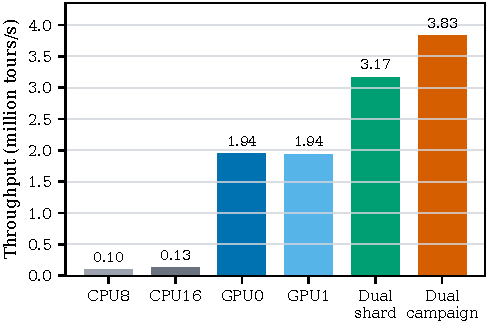
\includegraphics[width=\columnwidth]{accelerator_throughput.pdf}
\caption{正式加速基准的吞吐量。图内坐标保留英文。Campaign 为两个并发工作负载的总吞吐量。}
\label{fig:throughput-zh}
\end{figure}

单次运行的双 GPU 扩展率为 1.629。
它低于登记的 1.7 阈值。
两个独立运行的 campaign 扩展率为 1.972。
它高于登记的 1.8 阈值。
因此，独立任务并行更适合当前硬件。

平均 GPU 利用率约为 99\%。
峰值显存约为 286 MiB。
约 99.8\% 的热启动时间位于 CUDA kernel 内。
当前负载主要受计算能力限制。
继续增加缓存不太可能带来主要收益。

FP32 数值审计使用 TSP50 和 TSP100。
每个规模使用 128 个实例和三个配对 ACO 种子。
GPU 与 CPU 的平均参考差距之差为 \(-0.003445\) 个百分点。
单侧 95\% 上界为 0.000868 个百分点。
该值低于预设的 0.10 个百分点阈值。

\begin{table}[t]
\caption{三个 GP 运行的实测每代时间}
\label{tab:generation-time-zh}
\centering
\footnotesize
\begin{tabular}{lrr}
\toprule
变体 & 均值 \(\pm\) 标准差 (s) & 运行范围 (s)\\
\midrule
% 本文件由 build_paper_assets.py 生成，请勿手工修改。
AS & 34.50 $\pm$ 2.97 & 31.13--36.78 \\
ACS & 26.88 $\pm$ 4.43 & 21.97--30.57 \\
MMAS & 22.14 $\pm$ 3.34 & 18.31--24.41 \\
\bottomrule
%
\end{tabular}
\end{table}

\section{研究问题与结果分析}

\subsection{RQ1：无局部搜索时的有效性与泛化}

表~\ref{tab:main-results-zh} 报告每个 GP 运行的一个入选程序。
\(\Delta g<0\) 表示 RMTGP-ACO 更好。

\begin{table*}[t]
\caption{无局部搜索时，入选程序在均匀测试集上的结果。
CI 是 \(\Delta g\) 的分层 bootstrap 95\% 区间。
W/T/L 以百分比报告。}
\label{tab:main-results-zh}
\centering
\footnotesize
\begin{tabular}{lrrrrrl}
\toprule
ACO & \(n\) & Baseline 差距 (\%) & Full-F1 差距 (\%) &
\(\Delta g\) (pp) & 95\% CI (pp) & W/T/L\\
\midrule
% 本文件由 build_paper_assets.py 生成，请勿手工修改。
AS & 50 & 1.8803 & 1.7479 & -0.1324 & [-0.2076, -0.0718] & 54.7/2.8/42.4 \\
AS & 100 & 5.8952 & 4.2154 & -1.6799 & [-1.9680, -1.4739] & 92.1/0.0/7.9 \\
AS & 500 & 22.9874 & 15.1413 & -7.8461 & [-8.3979, -7.3727] & 100.0/0.0/0.0 \\
AS & 1000 & 30.4224 & 23.1088 & -7.3135 & [-8.5940, -6.1418] & 100.0/0.0/0.0 \\
ACS & 50 & 0.7326 & 0.6589 & -0.0736 & [-0.1050, -0.0432] & 46.6/17.6/35.9 \\
ACS & 100 & 1.9331 & 1.6412 & -0.2918 & [-0.3954, -0.2091] & 64.7/0.0/35.3 \\
ACS & 500 & 16.1641 & 12.9399 & -3.2242 & [-4.5698, -1.3932] & 93.8/0.0/6.2 \\
ACS & 1000 & 21.6293 & 19.2041 & -2.4252 & [-3.3961, -0.8317] & 94.8/0.0/5.2 \\
MMAS & 50 & 0.5941 & 0.4727 & -0.1215 & [-0.1549, -0.0820] & 52.3/22.4/25.2 \\
MMAS & 100 & 4.1088 & 1.8106 & -2.2982 & [-2.4240, -2.1223] & 99.2/0.0/0.8 \\
MMAS & 500 & 20.6291 & 14.1769 & -6.4522 & [-8.1652, -4.7067] & 100.0/0.0/0.0 \\
MMAS & 1000 & 25.4885 & 18.8571 & -6.6314 & [-8.3746, -4.8120] & 100.0/0.0/0.0 \\
\bottomrule
%
\end{tabular}
\end{table*}

\begin{figure*}[t]
\centering
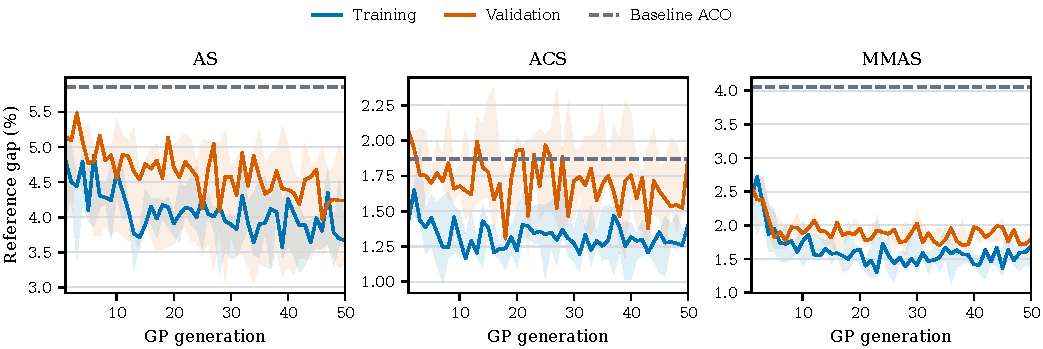
\includegraphics[width=\textwidth]{training_validation_curves.pdf}
\caption{无局部搜索的 TSP100 进化曲线。
每个运行在每代贡献一个代最佳个体。
实线是三个 GP 运行的中位数，阴影是最小值和最大值。}
\label{fig:training-curves-zh}
\end{figure*}

\begin{figure*}[t]
\centering
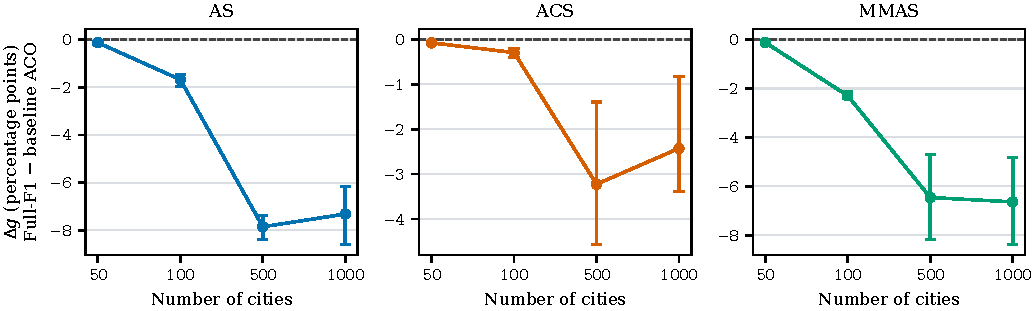
\includegraphics[width=\textwidth]{main_gap_delta.pdf}
\caption{Full-F1 与原始 ACO 的参考差距之差。
误差线为分层 bootstrap 95\% 区间。}
\label{fig:main-delta-zh}
\end{figure*}

12 个均值差及其区间均小于零。
下降幅度从 ACS 在 TSP50 上的 0.0736 个百分点，
到 AS 在 TSP500 上的 7.8461 个百分点。
三个 ACO 变体在训练时未见的 TSP500 和 TSP1000 上也得到改进。
曲线并非单调。
每代使用新的实例批量。
因此，入选检查点不一定来自最后一代。

\begin{table*}[t]
\caption{锁定分布偏移测试上的描述性结果。
所有测试使用相同的 TSP100 训练 Full-F1 champion。}
\label{tab:ood-results-zh}
\centering
\footnotesize
\begin{tabular}{llrrrl}
\toprule
ACO & 测试集 & Baseline 差距 (\%) & Full-F1 差距 (\%) &
\(\Delta g\) (pp) & W/T/L\\
\midrule
% 自动生成；OOD 不进行 terminal/function 因果推断。
AS & TSP500-C & 26.0627 & 19.7383 & -6.3245 & 100.0/0.0/0.0 \\
AS & TSP500-G & 20.0986 & 14.0184 & -6.0802 & 100.0/0.0/0.0 \\
AS & TSPLIB$\leq$500 & 10.0277 & 7.6313 & -2.3964 & 82.5/0.0/17.5 \\
ACS & TSP500-C & 16.3527 & 13.8345 & -2.5182 & 90.6/0.0/9.4 \\
ACS & TSP500-G & 14.8973 & 12.6798 & -2.2175 & 88.3/0.0/11.7 \\
ACS & TSPLIB$\leq$500 & 4.5376 & 3.5976 & -0.9399 & 77.8/0.0/22.2 \\
MMAS & TSP500-C & 22.7375 & 16.5961 & -6.1414 & 100.0/0.0/0.0 \\
MMAS & TSP500-G & 17.6609 & 12.1975 & -5.4635 & 100.0/0.0/0.0 \\
MMAS & TSPLIB$\leq$500 & 8.3755 & 5.0336 & -3.3419 & 93.7/2.4/4.0 \\
\bottomrule
%
\end{tabular}
\end{table*}

\begin{figure}[t]
\centering
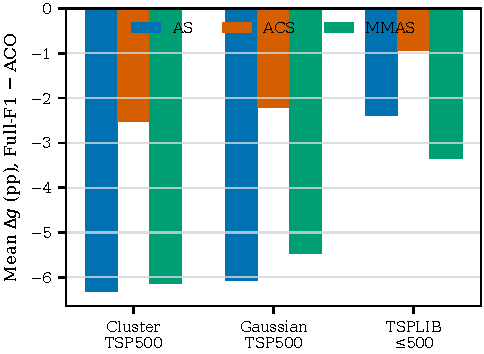
\includegraphics[width=\columnwidth]{ood_delta.pdf}
\caption{Cluster、Gaussian 和 TSPLIB 测试上的平均差距差值。
负值表示 Full-F1 更好。}
\label{fig:ood-delta-zh}
\end{figure}

九个 OOD 均值差均为负。
TSPLIB 胜率低于合成 OOD 数据。
AS、ACS 和 MMAS 的 TSPLIB 胜率分别为 82.5\%、77.8\% 和 93.7\%。
任何 OOD 分区都没有参与程序重选。

\textbf{对 RQ1 的回答：}
先导结果支持 Full-F1 相对原始 ACO 的改进，也支持跨规模迁移。
锁定 OOD 数据的均值也支持 Full-F1。
这一结果本身不能确定改进来自哪一个设计因素。

\subsection{RQ2：受控设计因素}

\begin{table*}[t]
\caption{31 节点预算下的主要受控对比。
每个单元格为估计值 [分层 bootstrap 95\% 区间]，单位为百分点。
负值支持列标题中前一个方法。}
\label{tab:ablation-primary-zh}
\centering
\scriptsize
\begin{tabular}{llrrr}
\toprule
ACO & 测试集 & TR-RGP \(-\) replacement &
Full-F1 \(-\) TR-RGP & Full-F1 \(-\) PH-RGP\\
\midrule
\input{paper_assets/ablation_primary_rows.tex}%
\end{tabular}
\end{table*}

\begin{figure*}[t]
\centering
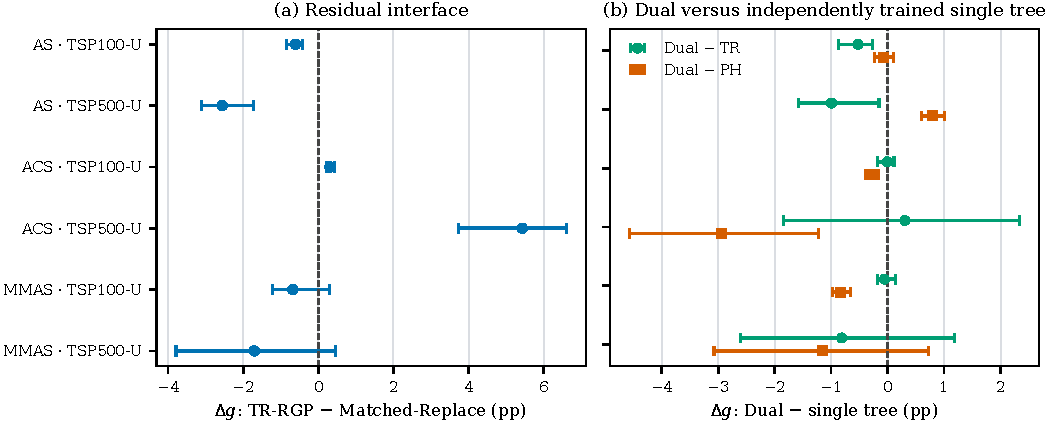
\includegraphics[width=\textwidth]{ablation_primary_forest.pdf}
\caption{残差接口与结构的主要受控对比。
负值分别支持残差接入或双树方法。}
\label{fig:ablation-primary-zh}
\end{figure*}

\begin{table*}[t]
\caption{与上一篇研究表示形式的同预算对比。
前两个数值列是平均最优差距。
最后一列是配对估计值 [分层 bootstrap 95\% 区间]，单位为百分点。
负值支持 Full-F1。}
\label{tab:legacy-comparison-zh}
\centering
\footnotesize
\begin{tabular}{llrrr}
\toprule
ACO & 测试集 & Legacy-GP 差距 (\%) & Full-F1 差距 (\%) &
Full-F1 $-$ Legacy-GP (pp)\\
\midrule
% 自动生成；Legacy-GP 与 Full-F1 均按当前实验预算重新训练。
AS & TSP100-U & 5.8952 & 4.2154 & -1.680 [-1.967, -1.473] \\
AS & TSP500-U & 22.9874 & 15.1413 & -7.846 [-8.423, -7.372] \\
ACS & TSP100-U & 1.9331 & 1.6412 & -0.292 [-0.395, -0.208] \\
ACS & TSP500-U & 16.1641 & 12.9399 & -3.224 [-4.576, -1.378] \\
MMAS & TSP100-U & 3.7469 & 1.8106 & -1.936 [-2.427, -1.458] \\
MMAS & TSP500-U & 27.0946 & 14.1769 & -12.918 [-20.080, -5.943] \\
\bottomrule
%
\end{tabular}
\end{table*}

\begin{figure}[t]
\centering
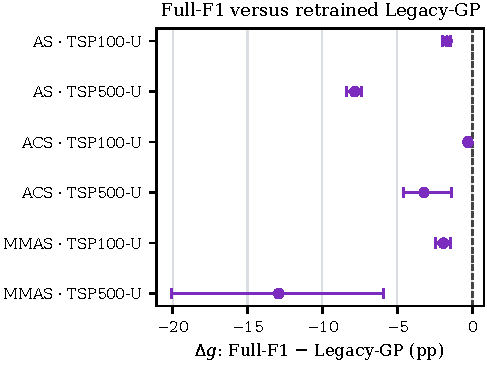
\includegraphics[width=\columnwidth]{legacy_comparison.pdf}
\caption{Full-F1 与重新训练的 Legacy-GP 之间的配对差值。
所有区间均低于零。}
\label{fig:legacy-comparison-zh}
\end{figure}

Full-F1 在六个上下文中的差距均低于重新训练的 Legacy-GP。
配对降幅为 0.2918 至 12.9177 个百分点。
所有区间均低于零。
这是两个完整表示方案之间的总体对比。
它不能单独识别残差接口、终端集或双树结构的作用。

AS 上的残差接入优于匹配的完整替换。
ACS 上则是完整替换更好。
MMAS 的两个区间都跨越零。
因此，残差方式不能被表述为普遍优于完整替换。
这也说明，有界残差与 MMAS 信息素上下界在形式上的相似性，
不足以构成机制结论。
二者限制的是不同变量。

在 31 节点预算下，Full-F1 没有在任何上下文中同时优于两个单树对照。
因子实验没有给出 Full 终端集的普遍优势。
它也没有给出 F1 函数集的普遍优势。
删除干预说明，两棵树会影响多个入选程序。
打乱干预没有显示稳定的运行内树对联合适应。
Full-F1 有效，但完整语法在部分上下文中可能设计过多。

\begin{figure*}[t]
\centering
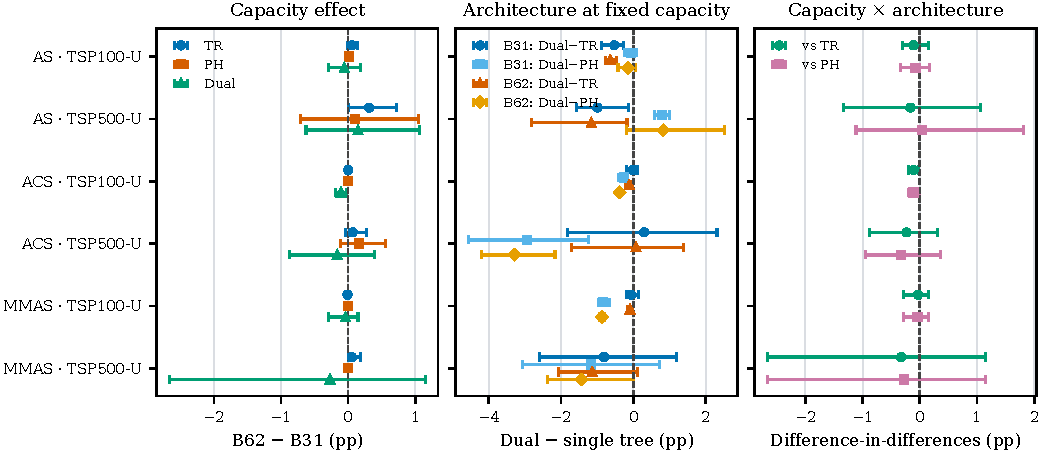
\includegraphics[width=\textwidth]{capacity_effects.pdf}
\caption{总节点预算为 31 和 62 时的容量与结构对比。
负值支持每个子图标题中的前一项。}
\label{fig:capacity-effects-zh}
\end{figure*}

容量实验包含 18 个结构内 B62 与 B31 对比。
只有一个 B62 减 B31 的区间完全小于零。
十个点估计为正。
入选表达式也很少接近节点上限。
对双树方法而言，B62 在 ACS TSP100 上使均值降低 0.1049 个百分点。
其余五个双树容量区间均跨越零。
额外表达式容量不是主要瓶颈。
B31 是更简约的默认设置。

\textbf{对 RQ2 的回答：}
结果支持在 AS 上使用残差接口，但不支持普遍结论。
当前完整表示在六个匹配上下文中均优于重新训练的上一篇研究表示。
这一比较不是组件层面的因果结果。
结果也不支持双树、Full 终端集或 F1 函数集具有一般优势。
两类语义角色都可能有作用。
收益取决于 ACO 变体和测试上下文。

\subsection{RQ3：训练实例数}

\begin{table*}[t]
\caption{ACS 训练实例预算实验。
每个单元格为平均差距 / \(\Delta g\)，单位为百分点。}
\label{tab:instance-budget-zh}
\centering
\footnotesize
\begin{tabular}{lrrrr}
\toprule
测试集 & Baseline & 32 个实例 & 64 个实例 & 128 个实例\\
\midrule
% Generated from the completed ACS instance-budget study.
TSP50-U & 0.7005 & 0.6544 / -0.0461 & 0.6501 / -0.0504 & 0.6757 / -0.0248 \\
TSP100-U & 1.9358 & 1.6106 / -0.3252 & 1.5977 / -0.3381 & 1.6258 / -0.3100 \\
TSP500-U & 16.0822 & 12.6558 / -3.4265 & 12.4316 / -3.6506 & 12.2874 / -3.7948 \\
TSP1000-U & 21.6125 & 19.1227 / -2.4898 & 18.8222 / -2.7903 & 18.7391 / -2.8734 \\
\bottomrule
%
\end{tabular}
\end{table*}

\begin{table}[t]
\caption{三个 GP 种子的单 GPU ACS 训练效率。
时间为均值 \(\pm\) 样本标准差。}
\label{tab:instance-budget-time-zh}
\centering
\footnotesize
\begin{tabular}{rrrr}
\toprule
实例数 & 每代时间 (s) & 总时间 (min) & 百万路线/s\\
\midrule
% Frozen summary of nine completed single-GPU runs; mean plus/minus sample SD.
32 & 7.63 $\pm$ 1.48 & 7.71 $\pm$ 1.24 & 6.44 $\pm$ 0.61 \\
64 & 10.43 $\pm$ 2.68 & 10.04 $\pm$ 2.26 & 7.57 $\pm$ 0.32 \\
128 & 17.21 $\pm$ 2.56 & 15.69 $\pm$ 2.15 & 9.36 $\pm$ 0.08 \\
\bottomrule
%
\end{tabular}
\end{table}

\begin{figure*}[t]
\centering
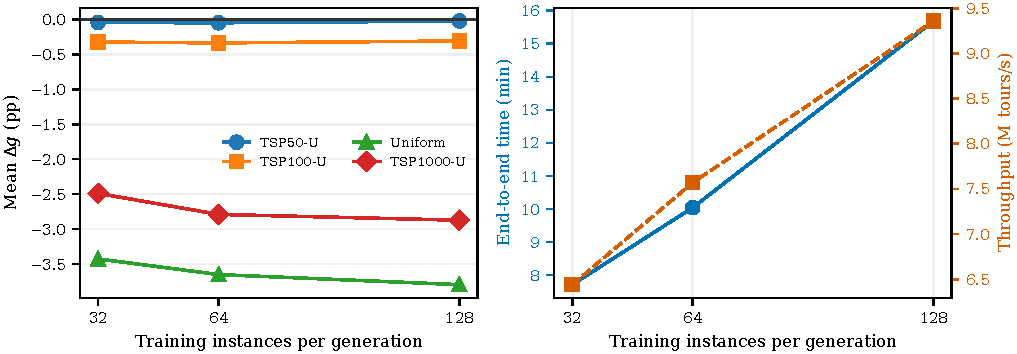
\includegraphics[width=\textwidth]{instance_budget_tradeoff.pdf}
\caption{每代使用 32、64 和 128 个训练实例时的质量、总时间与吞吐量。}
\label{fig:instance-budget-zh}
\end{figure*}

12 个“预算--测试集”均值都优于 baseline ACS。
64 个实例在 TSP50 和 TSP100 上最好。
128 个实例在 TSP500 和 TSP1000 上最好。
但是，每个条件只有三个 GP 种子。
不同种子的方向并不完全一致。
因此，这是随规模变化的趋势，不是显著的预算主效应。
批量从 32 增加到 128 时，吞吐量从每秒 644 万条路线提高到 936 万条。
端到端时间约增加一倍，而不是四倍。

\textbf{对 RQ3 的回答：}
较大批量提高 GPU 利用效率。
64 个实例给出较好的 TSP100 成本--质量折中。
128 个实例给出较好的大规模点估计。
三个种子的训练实例实验不能证明单纯增加训练数据一定产生更好的 GP 解。

\subsection{RQ4：2-opt 下的学习信号}

\begin{table}[t]
\caption{初始 TSP500 局部搜索实验。
数值为平均参考差距 (\%)。}
\label{tab:initial-ls-zh}
\centering
\footnotesize
\resizebox{\columnwidth}{!}{%
\begin{tabular}{lrrrr}
\toprule
ACO & ACO+2opt & RMTGP(no-LS)+2opt & RMTGP(LS)+2opt & ACO+3opt\\
\midrule
% Generated from the completed initial local-search study.
AS & 3.0117 & 2.6182 & 2.6609 & 1.8274 \\
ACS & 0.3114 & 0.2580 & 0.2588 & 0.1989 \\
MMAS & 0.0867 & 0.0939 & 0.0924 & 0.0304 \\
\bottomrule
%
\end{tabular}}
\end{table}

\begin{figure}[t]
\centering
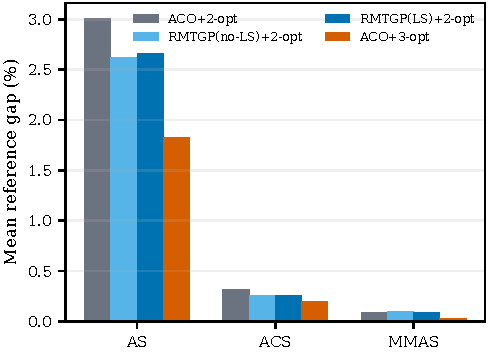
\includegraphics[width=\columnwidth]{initial_ls_tsp500_gap.pdf}
\caption{初始 TSP500 局部搜索实验。
只统计每个运行的最终入选程序。}
\label{fig:initial-ls-zh}
\end{figure}

第一轮局部搜索实验暴露了两个问题。
TSP100 在 2-opt 后接近饱和。
启用 2-opt 训练也没有稳定优于无局部搜索训练。
在 TSP500 上，AS 和 ACS 优于 ACO+2-opt，但仍差于 ACO+3-opt。
MMAS 没有优于 ACO+2-opt。

\begin{table*}[t]
\caption{500 次 ACO 迭代下的 TSP100 2-opt 信号审计。
Compression 是搜索后与搜索前的程序间方差比。
SNR 是程序间方差与种子内方差之比。
最后两列单位为百分比。}
\label{tab:signal-audit-zh}
\centering
\footnotesize
\begin{tabular}{lrrrrrrr}
\toprule
ACO & Baseline 差距 & Compression & Spearman &
最终 SNR & Basin SNR & 新增边 & 差异保留\\
\midrule
% Generated from the completed TSP100 2-opt signal audit at 500 ACO iterations.
AS & 0.2519 & 0.0347 & 0.940 & 0.100 & 35.811 & 21.1 & 33.5 \\
ACS & 0.1103 & 0.0108 & 0.660 & 0.113 & 1.239 & 9.4 & 35.4 \\
MMAS & 0.0270 & 0.0146 & 0.811 & 0.146 & 0.301 & 9.5 & 34.3 \\
\bottomrule
%
\end{tabular}
\end{table*}

\begin{figure*}[t]
\centering
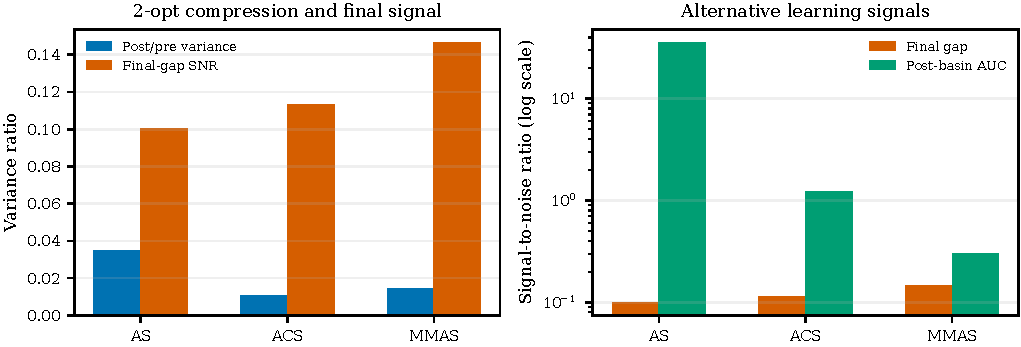
\includegraphics[width=\textwidth]{two_opt_signal_audit.pdf}
\caption{2-opt 后的方差压缩与信噪比。
右图使用对数坐标。}
\label{fig:signal-audit-zh}
\end{figure*}

AS、ACS 和 MMAS 在局部搜索后的方差分别只有搜索前的
3.47\%、1.08\% 和 1.46\%。
最终差距 SNR 最大只有 0.146。
AS 的搜索后盆地信号明显更强，ACS 也略有提高。
最终路线中约 9--21\% 的边由 2-opt 新加入。
构造差异只有约三分之一被保留。
这些结果支持使用盆地与 anytime 适应度。
它们也支持引入 \texttt{Origin}、\texttt{LSGain}、
\texttt{PreFreq} 和 \texttt{PostFreq}。
但是，它们不能证明某一个终端不可缺少。

\begin{table*}[t]
\caption{已完成的 TSP100 适应度对照在独立 512 实例 gate 上的结果。
数值是三个入选 GP 程序的均值。
Pass 表示部署 gate，不表示最终测试成功次数。}
\label{tab:tsp100-fitness-controls-zh}
\centering
\footnotesize
\begin{tabular}{llrrrrr}
\toprule
ACO & 适应度 & Baseline 差距 & Candidate 差距 & \(\Delta g\) &
差距下降 (\%) & Pass\\
\midrule
% Completed TSP100 fitness controls; independent 512-instance gate validation.
AS & Anytime+Final & 0.1301 & 0.1100 & -0.0201 & +15.4 & 3/3 \\
AS & Basin+Final & 0.1301 & 0.1341 & +0.0040 & -3.1 & 0/3 \\
ACS & Anytime+Final & 0.0448 & 0.0448 & +0.0000 & +0.0 & 0/3 \\
ACS & Basin+Final & 0.0448 & 0.0447 & -0.0001 & +0.2 & 0/3 \\
MMAS & Anytime+Final & 0.0173 & 0.0174 & +0.0001 & -0.4 & 0/3 \\
MMAS & Basin+Final & 0.0173 & 0.0186 & +0.0013 & -7.4 & 0/3 \\
\bottomrule
%
\end{tabular}
\end{table*}

\begin{figure*}[t]
\centering
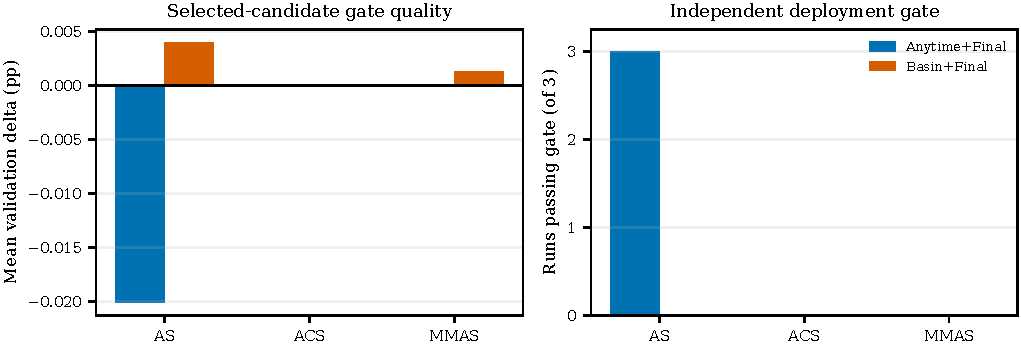
\includegraphics[width=\textwidth]{tsp100_fitness_controls.pdf}
\caption{已完成 TSP100 适应度对照的独立 gate 结果。
这些是验证结果，不能替代独立最终测试。}
\label{fig:tsp100-fitness-controls-zh}
\end{figure*}

Anytime+Final 对照通过三个 AS 部署 gate，并使 AS 验证差距降低 15.4\%。
ACS 和 MMAS 没有得到对应收益。
Basin+Final 对照没有通过任何 gate。
这说明，仅替换为更密集的适应度并不足以解决问题。
该结果也支持把下一阶段训练从接近饱和的 TSP100 移到 TSP500。

\begin{table*}[t]
\caption{16 个实例、500 次迭代下的严格 TSP500 racing 审计。
登记阈值为 SNR \(\geq1\)、recall \(\geq0.8\) 和 Spearman
\(\geq0.7\)，并同时检查非零响应。}
\label{tab:tsp500-racing-audit-zh}
\centering
\footnotesize
\begin{tabular}{lrrrrrl}
\toprule
ACO & Final 非零 & Anytime 非零 & Combined SNR &
Top-32 recall & Spearman & Pass\\
\midrule
% TSP500 racing audit at the fixed 16-instance, 500-iteration screen.
AS & 0.952 & 0.952 & 0.651 & 0.938 & 0.959 & No \\
ACS & 0.890 & 0.906 & 0.278 & 0.719 & 0.640 & No \\
MMAS & 0.813 & 0.844 & 0.290 & 0.719 & 0.578 & No \\
\bottomrule
%
\end{tabular}
\end{table*}

\begin{figure*}[t]
\centering
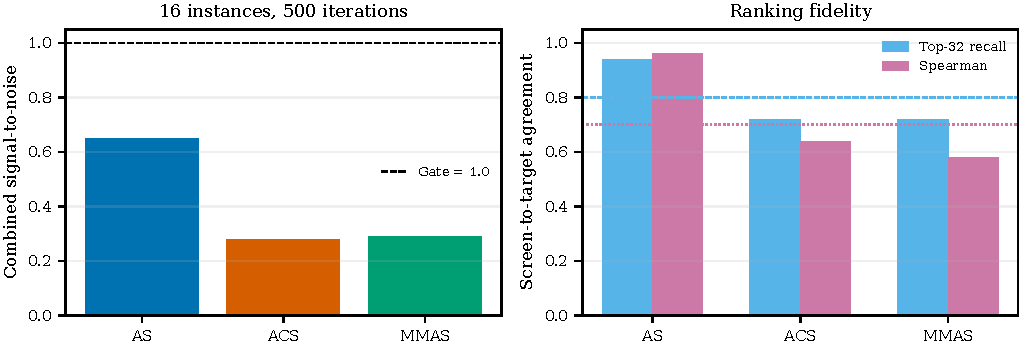
\includegraphics[width=\textwidth]{tsp500_racing_audit.pdf}
\caption{严格 TSP500 筛选的信号与排序诊断。
三个变体都没有达到登记的 SNR 阈值。}
\label{fig:tsp500-racing-audit-zh}
\end{figure*}

该筛选产生了较多非零响应，但三个变体的 SNR 均小于一。
AS 的排序一致性达到阈值。
ACS 和 MMAS 还没有达到 recall 与相关性阈值。
因此，该协议没有启动正式 racing 训练。
最终 v2 流程用逐步增大的高保真批量替代小规模固定筛选，
最大使用 128 个实例和三个种子。

\textbf{对 RQ4 的回答：}
2-opt 压缩最终差距信号，并删除大量构造差异。
只使用最终差距作为训练目标时，区分度较弱。
信号审计为盆地/anytime 信息提供依据。
已完成对照表明，只改变适应度仍不充分。
小筛选 gate 的失败支持更大的分阶段高保真设计。
单个终端的因果作用仍未被隔离。

\subsection{RQ5：TSP500 局部搜索感知质量与时间}

\begin{figure*}[t]
\centering
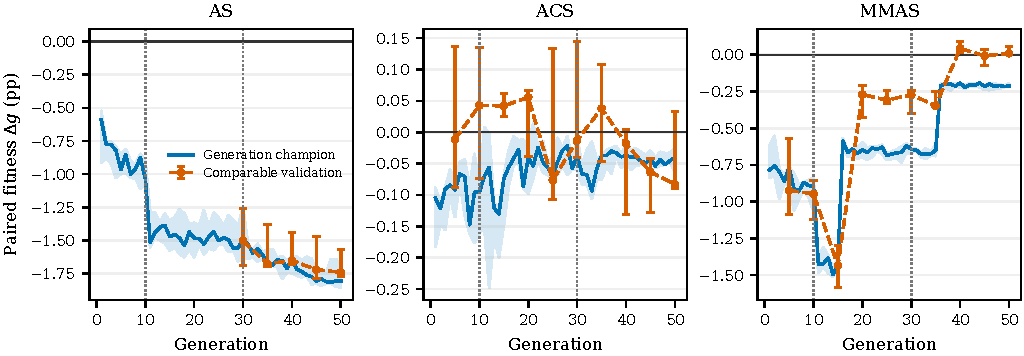
\includegraphics[width=\textwidth]{ls_v2_training_curves.pdf}
\caption{TSP500 局部搜索感知训练曲线。
每个运行贡献代最佳个体。
实线为三个 GP 种子的中位数，阴影为范围。
竖线表示第 10 代和第 30 代。
只有三个运行使用相同 ACO 迭代数的验证点才被合并。}
\label{fig:ls-training-zh}
\end{figure*}

\begin{table*}[t]
\caption{最终 TSP500 局部搜索感知测试。
U95 是相对 ACO+2-opt 的单侧 95\% 上界。
最后一列依次表示是否满足对 ACO+2-opt 的登记成功条件，
以及是否优于 ACO+3-opt。}
\label{tab:ls-v2-main-zh}
\centering
\scriptsize
\resizebox{\textwidth}{!}{%
\begin{tabular}{llrrrrrrl}
\toprule
ACO & 分布 & ACO+2opt 差距 & RMTGP+2opt 差距 &
\(\Delta_2\) & U95\(_2\) & ACO+3opt 差距 & \(\Delta_3\) &
Success\(_2\)/Better\(_3\)\\
\midrule
% Generated from the completed TSP500 LS-aware v2 final test.
AS & Uniform & 3.0662 & 1.3554 & -1.7109 & -1.6368 & 1.7908 & -0.4355 & Yes/Yes \\
AS & Cluster & 3.0344 & 2.0609 & -0.9735 & -0.8820 & 1.4769 & +0.5839 & Yes/No \\
AS & Gaussian & 2.7789 & 1.3889 & -1.3900 & -1.3082 & 1.7618 & -0.3728 & Yes/Yes \\
ACS & Uniform & 0.3221 & 0.2951 & -0.0270 & +0.0056 & 0.1846 & +0.1105 & No/No \\
ACS & Cluster & 0.2558 & 0.2593 & +0.0035 & +0.0498 & 0.1148 & +0.1444 & No/No \\
ACS & Gaussian & 0.2891 & 0.2937 & +0.0046 & +0.0364 & 0.2082 & +0.0855 & No/No \\
MMAS & Uniform & 0.0808 & 0.1021 & +0.0213 & +0.0333 & 0.0367 & +0.0654 & No/No \\
MMAS & Cluster & 0.0682 & 0.0666 & -0.0016 & +0.0103 & 0.0202 & +0.0464 & No/No \\
MMAS & Gaussian & 0.1382 & 0.1341 & -0.0041 & +0.0078 & 0.0606 & +0.0735 & No/No \\
\bottomrule
%
\end{tabular}}
\end{table*}

\begin{figure*}[t]
\centering
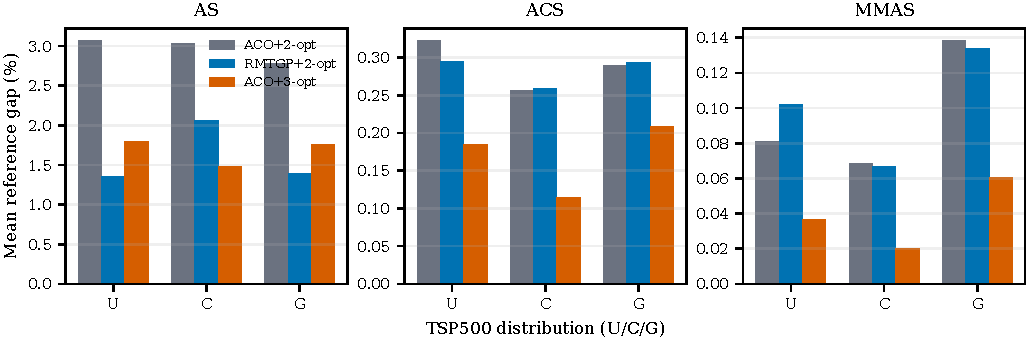
\includegraphics[width=\textwidth]{ls_v2_gap_comparison.pdf}
\caption{均匀、聚类和高斯 TSP500 上的最终平均差距。}
\label{fig:ls-gap-zh}
\end{figure*}

AS 在三个分布上都满足相对 ACO+2-opt 的登记成功条件。
差距分别下降 1.7109、0.9735 和 1.3900 个百分点。
它在均匀和高斯 TSP500 上也优于 ACO+3-opt。
在聚类 TSP500 上，它比 ACO+3-opt 高 0.5839 个百分点。
三个 AS GP 运行均优于 ACO+2-opt。

ACS 在均匀集上只有很小改进。
其单侧上界跨越零，且相对下降不到 10\%。
在聚类集和高斯集上，ACS 均值略差于 ACO+2-opt。
MMAS 在均匀集上更差，在另外两个分布上差异很小。
ACS 和 MMAS 均未通过登记 gate。

\begin{table}[t]
\caption{三个 TSP500 分布上的描述性均值}
\label{tab:ls-v2-pooled-zh}
\centering
\scriptsize
\resizebox{\columnwidth}{!}{%
\begin{tabular}{lrrrrrr}
\toprule
ACO & ACO2 & RMTGP2 & ACO3 & \(\Delta_2\) & \(\Delta_3\) &
差距下降 (\%)\\
\midrule
% Descriptive arithmetic means across the three TSP500 distributions.
AS & 2.9599 & 1.6017 & 1.6765 & -1.3581 & -0.0748 & +45.9 \\
ACS & 0.2890 & 0.2827 & 0.1692 & -0.0063 & +0.1135 & +2.2 \\
MMAS & 0.0957 & 0.1010 & 0.0392 & +0.0052 & +0.0618 & -5.5 \\
\bottomrule
%
\end{tabular}}
\end{table}

\begin{figure*}[t]
\centering
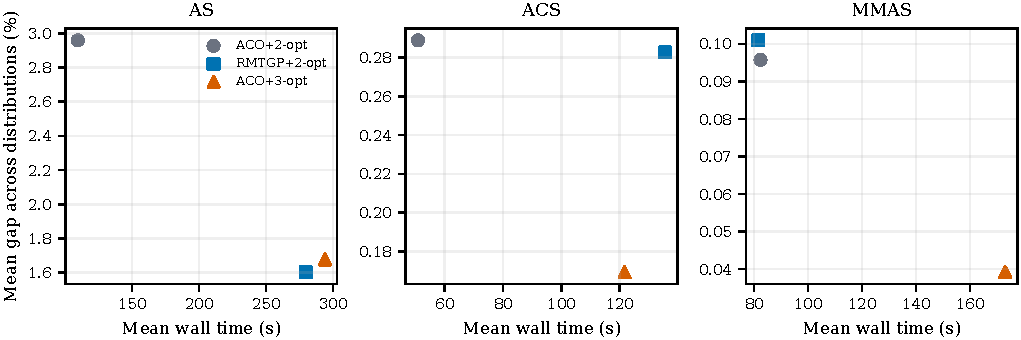
\includegraphics[width=\textwidth]{ls_v2_runtime_quality.pdf}
\caption{三个 TSP500 分布上的最终入选程序平均运行时间与平均差距。
每个点表示一种策略在三个分布上的均值。}
\label{fig:ls-runtime-zh}
\end{figure*}

AS 的 RMTGP+2-opt 平均运行时间接近 ACO+3-opt。
它在聚类集上更快，在均匀集上相同，在高斯集上略慢。
MMAS 的 RMTGP+2-opt 比 ACO+3-opt 快 1.97--2.29 倍，
但其质量更差。
因此，时间节省与质量变化必须同时报告。

\textbf{对 RQ5 的回答：}
局部搜索感知方法在 AS 上取得成功。
它在三个分布上均优于 ACO+2-opt，并在两个分布上优于 ACO+3-opt。
ACS 和 MMAS 不支持相同结论。
因此，“RMTGP+2-opt 达到 ACO+3-opt”只对特定 AS 分布成立。

\subsection{RQ6：计算效率}

\begin{figure}[t]
\centering
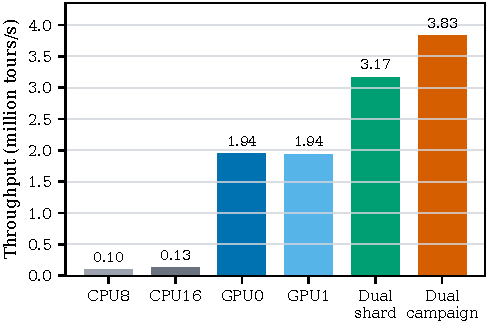
\includegraphics[width=\columnwidth]{accelerator_throughput.pdf}
\caption{登记的 RTX 4000 Ada 种群训练吞吐量。
数值相对 16 线程 CPU 实现。}
\label{fig:accelerator-zh}
\end{figure}

融合评估器相对 CPU16 取得 14.626 倍单 GPU 加速。
双 GPU 分片取得 23.820 倍加速。
两个独立运行并发取得 1.972 倍 campaign 扩展。
这些值只适用于登记的 RTX 4000 Ada 工作负载。

\begin{table*}[t]
\caption{已完成 TSP500 局部搜索感知训练的时间。
数值为三个 GP 运行的均值 \(\pm\) 样本标准差。
阶段列的单位为每代秒数。}
\label{tab:ls-training-time-zh}
\centering
\footnotesize
\begin{tabular}{lrrrrr}
\toprule
ACO & 总时间 (h) & G1--15 & G16--35 & G36--50 & 后期百万路线/s\\
\midrule
% TSP500 LS-aware v2 training time; mean plus/minus sample SD over three GP runs.
AS & 14.83 $\pm$ 5.61 & 117.1 $\pm$ 66.3 & 454.1 $\pm$ 283.6 & 2837.3 $\pm$ 1677.6 & 0.14 $\pm$ 0.07 \\
ACS & 2.92 $\pm$ 0.60 & 24.9 $\pm$ 0.4 & 80.6 $\pm$ 4.4 & 569.5 $\pm$ 146.4 & 0.53 $\pm$ 0.12 \\
MMAS & 2.63 $\pm$ 0.20 & 35.7 $\pm$ 1.6 & 100.2 $\pm$ 5.3 & 460.9 $\pm$ 54.2 & 0.63 $\pm$ 0.06 \\
\bottomrule
%
\end{tabular}
\end{table*}

\begin{figure*}[t]
\centering
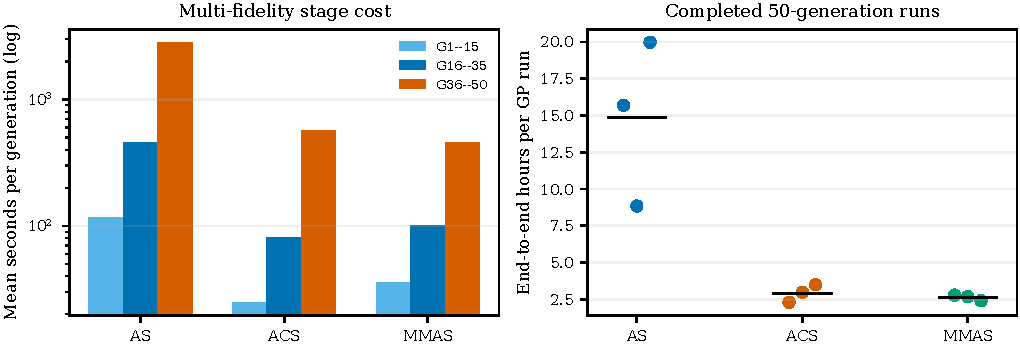
\includegraphics[width=\textwidth]{ls_v2_training_time.pdf}
\caption{九个已完成 TSP500 局部搜索感知 GP 运行的阶段时间与端到端时间。}
\label{fig:ls-training-time-zh}
\end{figure*}

\begin{table}[t]
\caption{已完成 TSP500 campaign 的时间核算}
\label{tab:ls-campaign-time-zh}
\centering
\scriptsize
\resizebox{\columnwidth}{!}{%
\begin{tabular}{llll}
\toprule
阶段 & 工作量 & 时间 & 口径\\
\midrule
% End-to-end completed TSP500 LS-aware campaign accounting.
Training & 9 GP runs & 61.15 GPU-h & Sum of recorded run wall times \\
Final test & 27 shards & 3.34 wall-h & 2 GPUs; includes latency audit \\
\bottomrule
%
\end{tabular}}
\end{table}

保真度逐步增加后，后期每代时间明显上升。
AS、ACS 和 MMAS 的平均端到端时间分别为
14.83、2.92 和 2.63 小时。
AS 每轮包含 32 个增强事件，而 ACS 与 MMAS 只有一个。
不同入选表达式使用的重语义路径也不同。
当前计时没有隔离这些原因。
九次训练合计记录 61.15 GPU 小时。
最终测试只评估入选程序，共包含 27 个独立 shard。
两张 GPU 在 3.34 小时内完成测试和 latency audit。

\begin{table}[t]
\caption{RTX PRO 5000 Blackwell 局部搜索 kernel 微基准}
\label{tab:blackwell-kernels-zh}
\centering
\scriptsize
\resizebox{\columnwidth}{!}{%
\begin{tabular}{lrl}
\toprule
优化 & 加速比 & 对照\\
\midrule
% Blackwell implementation microbenchmarks; protocols differ and are not combined statistically.
2-opt launch: 8 vs. 4 warps & 1.045$\times$ & ACS, TSP100, 64 instances, population 100, 10 ACO iterations \\
3-opt block: 512 threads, TSP100 & 1.909$\times$ & old one-warp kernel \\
3-opt block: 512 threads, TSP500 & 3.511$\times$ & old one-warp kernel \\
Edge LSGain matrix path & 25.640$\times$ & old per-edge loop \\
\bottomrule
%
\end{tabular}}
\end{table}

\begin{figure}[t]
\centering
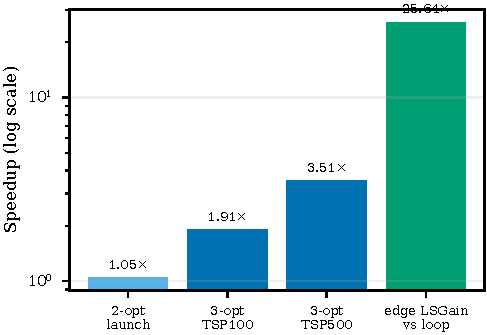
\includegraphics[width=\columnwidth]{blackwell_kernel_speedups.pdf}
\caption{Blackwell kernel 加速比。
各项使用不同协议，因此不合并进行统计比较。}
\label{fig:blackwell-zh}
\end{figure}

每个 block 使用八个 2-opt warp 后，入选 launch 加速 1.045 倍。
512-thread 3-opt kernel 相对旧 warp kernel，
在 TSP100 和 TSP500 上分别加速 1.909 倍与 3.511 倍。
紧凑 edge-\texttt{LSGain} 路径比旧逐边循环快 25.64 倍。
在独立语义微基准中，矩阵化频数终端增加不到 1\% 的开销。
较重的 \texttt{LSGain} 路径仍比轻量路径多 38.4\% 开销。
这一结果支持按终端语义分片。

\textbf{对 RQ6 的回答：}
“程序--实例”融合使嵌套 GP--ACO 训练可行。
大实例批量提高设备占用率。
TSP500 实验还依赖紧凑局部搜索状态、语义分片、常驻缓存和多 GPU shard 调度。
完整实验实测使用 61.15 GPU 小时训练，并用两张 GPU 在 3.34 小时内完成最终测试。
不同 GPU 型号上的硬件加速比不能直接相互转移。

\section{局限性与有效性威胁}

每个进化条件只有三个 GP 运行。
分层 bootstrap 包含多个实例和 ACO 种子，
但不能代替更多独立进化运行。
因此，消融、容量和训练实例预算结论均为先导证据。

无局部搜索实验在均匀 TSP100 上训练。
局部搜索感知实验在均匀 TSP500 上训练。
分布迁移只使用两类合成分布和一个较小的 TSPLIB 子集。
当前方法只实现 AS、同步 ACS 和使用所列参数的 MMAS。

局部搜索感知验证曲线包含一次恢复记录差异。
AS 的五个早期监测代在不同种子间使用了不同 ACO 迭代数。
这些点没有进入合并验证曲线。
它们不影响育种或最终测试。
全部最终比较均使用 5000 次迭代和每个运行的入选程序。

最终局部搜索感知语法同时改变了训练规模、容量、终端、适应度和分阶段策略。
因此，最终结果不能单独归因到 \texttt{LSGain}、其他某一个终端或阶段计划。
ACS 和 MMAS 的失败也说明该扩展没有普遍效果。

参考路线有效，但数据没有为每条路线附带全局最优性证书。
因此，本文使用“参考差距”而非“最优差距”。
GPU 搜索使用 FP32-fast，最终路线长度使用 FP64 重算。
不同后端不要求离散 ACO 路径逐位相同。

训练吞吐量与单程序延迟是两类不同负载。
RTX 4000 Ada、RTX A5000 和 RTX PRO 5000 Blackwell 的结果不能合并为一个硬件比较。

\section{结论}

RMTGP-ACO 进化两个强类型残差程序。
状态转移树修正原始选择分数。
信息素树重新分配原始增强预算。
两棵树输出零时恢复原始 ACO。

无局部搜索时，Full-F1 在 12 个均匀“变体--规模”比较中均降低平均差距。
它还在六个匹配的 TSP100/TSP500 上下文中优于重新训练的 Legacy-GP。
后一结果比较的是完整表示，而不是单个组件。
控制实验对这一结果给出重要限定。
残差接入并不总是优于完整替换。
双树并不总是优于两个单树对照。
较丰富的终端与函数配置也不总是有用。
把总节点预算从 31 增加到 62 同样不是一般性的解决方案。

2-opt 信号审计指出另一个问题。
局部搜索会压缩最终差距信号。
因此，局部搜索感知扩展使用边来源和移动信息、多保真适应度，
并在 TSP500 上分阶段进化。
该扩展对 AS 有效。
它在三个测试分布上都优于 ACO+2-opt，
并在其中两个分布上优于 ACO+3-opt。
同一结论不适用于 ACS 或 MMAS。

CUDA 实现使这些嵌套实验可执行。
主要工程改进包括“程序--实例”融合、紧凑局部搜索状态、
生成式 GP kernel、语义分片、baseline 缓存和多 GPU 任务调度。
后续工作应增加独立 GP 运行数，并逐一隔离局部搜索感知设计因素。

\appendices

\section{完整控制消融表}

\begin{table}[h]
\caption{残差状态转移减去匹配完整替换 (pp)}
\label{tab:appendix-residual-zh}
\centering
\scriptsize
\resizebox{\columnwidth}{!}{%
\begin{tabular}{llr}
\toprule
ACO & 测试集 & 估计值 [95\% CI]\\
\midrule
% 自动生成；负值表示 residual 接口具有更低 gap。
AS & TSP100-U & -0.606 [-0.853, -0.413] \\
AS & TSP500-U & -2.558 [-3.119, -1.720] \\
ACS & TSP100-U & +0.311 [+0.216, +0.436] \\
ACS & TSP500-U & +5.430 [+3.726, +6.602] \\
MMAS & TSP100-U & -0.679 [-1.224, +0.291] \\
MMAS & TSP500-U & -1.706 [-3.790, +0.452] \\
\bottomrule
%
\end{tabular}}
\end{table}

\begin{table}[h]
\caption{31 节点下双树减去单树对照 (pp)}
\label{tab:appendix-architecture-zh}
\centering
\scriptsize
\resizebox{\columnwidth}{!}{%
\begin{tabular}{llrr}
\toprule
ACO & 测试集 & Full-F1 \(-\) TR & Full-F1 \(-\) PH\\
\midrule
% 自动生成；负值表示 31 节点双树具有更低 gap。
AS & TSP100-U & -0.525 [-0.876, -0.265] & -0.068 [-0.230, +0.100] \\
AS & TSP500-U & -0.994 [-1.580, -0.153] & +0.795 [+0.597, +1.007] \\
ACS & TSP100-U & -0.006 [-0.179, +0.113] & -0.263 [-0.393, -0.167] \\
ACS & TSP500-U & +0.304 [-1.843, +2.336] & -2.950 [-4.575, -1.219] \\
MMAS & TSP100-U & -0.056 [-0.182, +0.144] & -0.828 [-0.970, -0.659] \\
MMAS & TSP500-U & -0.810 [-2.601, +1.187] & -1.162 [-3.075, +0.731] \\
\bottomrule
%
\end{tabular}}
\end{table}

\begin{table*}[h]
\caption{Core/Full 与 F0/F1 因子效应 (pp)}
\label{tab:appendix-factorial-zh}
\centering
\scriptsize
\resizebox{\textwidth}{!}{%
\begin{tabular}{llrrr}
\toprule
ACO & 测试集 & Full \(-\) Core & F1 \(-\) F0 & 交互效应\\
\midrule
% 自动生成；负值表示相应线性 contrast 降低 gap。
AS & TSP100-U & -0.213 [-0.534, +0.021] & +0.501 [-0.254, +0.990] & -0.410 [-0.900, +0.406] \\
AS & TSP500-U & -0.414 [-1.433, +0.844] & +0.951 [+0.066, +2.504] & -1.953 [-5.492, +1.437] \\
ACS & TSP100-U & -0.030 [-0.122, +0.071] & -0.022 [-0.058, +0.016] & -0.005 [-0.063, +0.057] \\
ACS & TSP500-U & +0.210 [-1.043, +2.296] & -0.219 [-1.197, +0.373] & +0.074 [-0.383, +0.548] \\
MMAS & TSP100-U & +0.085 [+0.017, +0.155] & +0.033 [-0.042, +0.143] & -0.004 [-0.215, +0.186] \\
MMAS & TSP500-U & +0.528 [+0.080, +1.163] & +0.353 [-1.106, +1.365] & +0.549 [-1.514, +2.519] \\
\bottomrule
%
\end{tabular}}
\end{table*}

\begin{table*}[h]
\caption{树删除与跨运行配对干预 (pp)}
\label{tab:appendix-mechanism-zh}
\centering
\scriptsize
\resizebox{\textwidth}{!}{%
\begin{tabular}{llrrrr}
\toprule
ACO & 测试集 & Full \(-\) drop-TR & Full \(-\) drop-PH &
Full \(-\) shuffle-1 & Full \(-\) shuffle-2\\
\midrule
% 自动生成；负值表示原始 Full-F1 配对更好。
AS & TSP100-U & -0.270 [-0.728, +0.000] & -1.290 [-1.576, -1.058] & -0.214 [-0.349, -0.097] & -0.292 [-0.735, +0.211] \\
AS & TSP500-U & -1.824 [-5.132, +0.000] & -6.090 [-7.765, -3.058] & -0.666 [-5.459, +2.957] & -0.749 [-5.407, +3.422] \\
ACS & TSP100-U & -0.273 [-0.321, -0.222] & -0.018 [-0.091, +0.048] & -0.032 [-0.092, +0.039] & -0.007 [-0.147, +0.121] \\
ACS & TSP500-U & -2.817 [-4.044, -0.854] & -0.341 [-0.659, -0.019] & -0.116 [-0.598, +0.273] & -0.236 [-0.540, +0.110] \\
MMAS & TSP100-U & -1.534 [-2.102, -1.006] & -0.134 [-0.255, +0.000] & +0.014 [-0.254, +0.239] & +0.026 [-0.135, +0.250] \\
MMAS & TSP500-U & -4.403 [-4.679, -4.140] & -1.551 [-2.834, +0.000] & -0.027 [-1.769, +2.845] & -0.029 [-2.834, +1.633] \\
\bottomrule
%
\end{tabular}}
\end{table*}

\begin{figure*}[h]
\centering

\includegraphics[width=\textwidth]{factorial_effects.pdf}
\caption{完整因子对比。
没有交互效应区间排除零。}
\label{fig:appendix-factorial-zh}
\end{figure*}

\begin{figure*}[h]
\centering
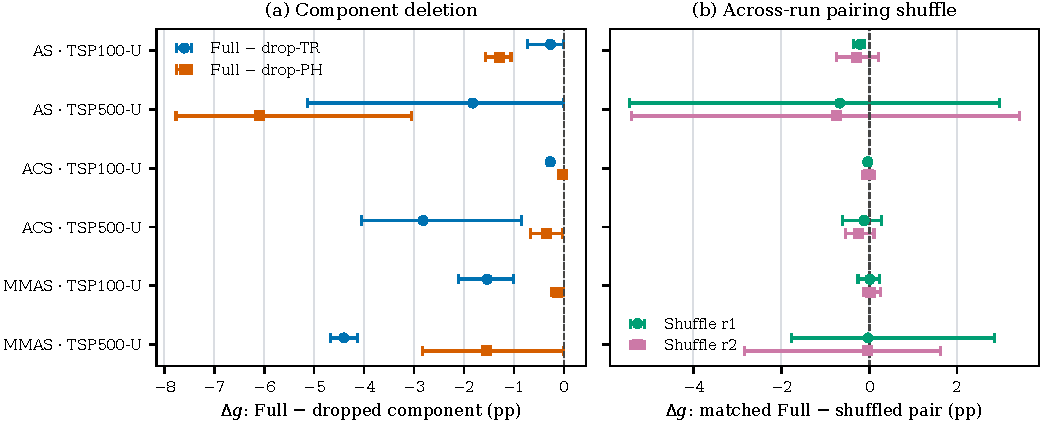
\includegraphics[width=\textwidth]{mechanism_effects.pdf}
\caption{完整的训练后删除与打乱配对对比。}
\label{fig:appendix-mechanism-zh}
\end{figure*}

\begin{table*}[h]
\caption{B31 与 B62 下的容量和结构对比}
\label{tab:appendix-capacity-zh}
\centering
\scriptsize
\resizebox{\textwidth}{!}{%
\begin{tabular}{llrrrrr}
\toprule
ACO & 测试集 & B62\(-\)B31 & B31 Full\(-\)TR &
B31 Full\(-\)PH & B62 Full\(-\)TR & B62 Full\(-\)PH\\
\midrule
% 自动生成；负值表示公式前项具有更低 gap。
AS & TSP100-U & -0.055 [-0.290, +0.183] & -0.525 [-0.873, -0.260] & -0.068 [-0.228, +0.102] & -0.635 [-0.756, -0.470] & -0.143 [-0.421, +0.050] \\
AS & TSP500-U & +0.148 [-0.627, +1.062] & -0.994 [-1.580, -0.142] & +0.795 [+0.593, +1.003] & -1.160 [-2.826, -0.173] & +0.835 [-0.195, +2.523] \\
ACS & TSP100-U & -0.105 [-0.194, -0.023] & -0.006 [-0.185, +0.112] & -0.263 [-0.398, -0.167] & -0.114 [-0.219, -0.022] & -0.373 [-0.420, -0.323] \\
ACS & TSP500-U & -0.163 [-0.875, +0.400] & +0.304 [-1.819, +2.315] & -2.950 [-4.561, -1.241] & +0.073 [-1.707, +1.393] & -3.281 [-4.189, -2.165] \\
MMAS & TSP100-U & -0.040 [-0.292, +0.147] & -0.056 [-0.184, +0.142] & -0.828 [-0.971, -0.663] & -0.088 [-0.149, -0.025] & -0.868 [-0.945, -0.802] \\
MMAS & TSP500-U & -0.271 [-2.665, +1.153] & -0.810 [-2.582, +1.200] & -1.162 [-3.061, +0.730] & -1.138 [-2.059, +0.123] & -1.433 [-2.375, +0.000] \\
\bottomrule
%
\end{tabular}}
\end{table*}

\begin{table}[h]
\caption{B31/B62 入选程序的节点数中位数}
\label{tab:appendix-capacity-nodes-zh}
\centering
\scriptsize
\begin{tabular}{lrrr}
\toprule
ACO & TR-RGP & PH-RGP & Full-F1\\
\midrule
% 自动生成；每项为 B31 champion / B62 champion 节点中位数。
AS & 17/15 & 19/16 & 27/31 \\
ACS & 12/15 & 5/6 & 17/20 \\
MMAS & 19/19 & 7/7 & 19/20 \\
\bottomrule
%
\end{tabular}
\end{table}

\begin{figure}[h]
\centering
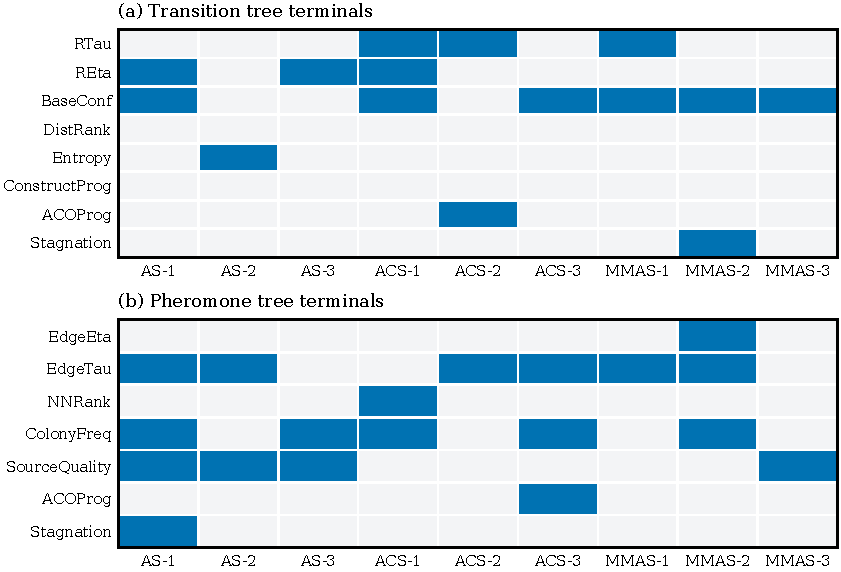
\includegraphics[width=\columnwidth]{terminal_usage_heatmap.pdf}
\caption{九个无局部搜索 Full-F1 champion 的终端语法使用情况。}
\label{fig:appendix-terminal-use-zh}
\end{figure}

\section{局部搜索开发实验}

\begin{table*}[h]
\caption{完整的初始局部搜索结果。
数值为平均参考差距 (\%)，只使用每个运行的最终入选程序。}
\label{tab:appendix-initial-ls-zh}
\centering
\footnotesize
\begin{tabular}{llrrrr}
\toprule
ACO & 测试集 & ACO+2opt & RMTGP(no-LS)+2opt &
RMTGP(LS)+2opt & ACO+3opt\\
\midrule
% Full initial local-search results; final candidates only.
AS & TSP100-U & 0.0300 & 0.0311 & 0.0312 & 0.0043 \\
AS & Uniform & 3.0117 & 2.6182 & 2.6609 & 1.8274 \\
ACS & TSP100-U & 0.0154 & 0.0072 & 0.0028 & 0.0037 \\
ACS & Uniform & 0.3114 & 0.2580 & 0.2588 & 0.1989 \\
MMAS & TSP100-U & 0.0015 & 0.0007 & 0.0010 & 0.0007 \\
MMAS & Uniform & 0.0867 & 0.0939 & 0.0924 & 0.0304 \\
\bottomrule
%
\end{tabular}
\end{table*}

信号先导实验比较最终差距、盆地分数与组合适应度。
它们还检查残差半径和 \texttt{Origin} 终端。
这些实验只运行三代，用于选择开发方向。
它们不是确认性的终端消融。
失败的严格 TSP500 racing gate 也只作为诊断证据。
它推动了 128 个训练实例、更长 ACO 迭代数和最终 v2 协议。
任何不完整 shard 都没有进入主表。

\section{TSP500 运行时间与入选程序}

\begin{table*}[h]
\caption{TSP500 最终入选程序的运行时间，单位为秒。
最后一列是 ACO+3opt 时间除以 RMTGP+2opt 时间。}
\label{tab:appendix-ls-runtime-zh}
\centering
\footnotesize
\begin{tabular}{llrrrr}
\toprule
ACO & 分布 & ACO+2opt & RMTGP+2opt & ACO+3opt & 比值\\
\midrule
% Generated from the TSP500 LS-aware v2 latency audit; one selected program.
AS & Uniform & 108.4 & 264.3 & 264.3 & 1.00 \\
AS & Cluster & 113.3 & 288.9 & 344.4 & 1.19 \\
AS & Gaussian & 107.3 & 285.9 & 273.4 & 0.96 \\
ACS & Uniform & 36.7 & 72.6 & 83.6 & 1.15 \\
ACS & Cluster & 69.0 & 204.5 & 171.4 & 0.84 \\
ACS & Gaussian & 47.0 & 129.7 & 110.1 & 0.85 \\
MMAS & Uniform & 76.8 & 73.4 & 144.9 & 1.97 \\
MMAS & Cluster & 91.9 & 91.8 & 210.6 & 2.29 \\
MMAS & Gaussian & 78.5 & 79.4 & 163.6 & 2.06 \\
\bottomrule
%
\end{tabular}
\end{table*}

\begin{figure*}[h]
\centering
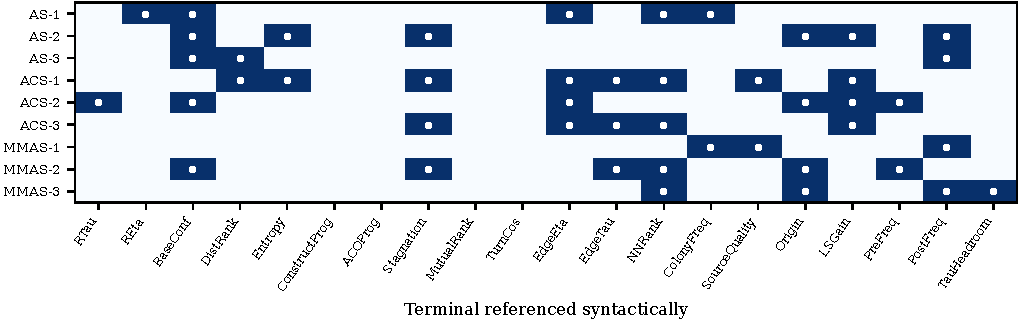
\includegraphics[width=\textwidth]{ls_v2_terminal_usage.pdf}
\caption{九个 TSP500 局部搜索感知入选程序的终端语法使用情况。
出现次数不是因果效应。}
\label{fig:appendix-ls-terminals-zh}
\end{figure*}

\begin{table*}[h]
\caption{入选的 TSP500 局部搜索感知表达式。
Hash 标识序列化候选程序。}
\label{tab:appendix-expressions-zh}
\centering
\scriptsize
\begin{tabular}{llp{0.74\textwidth}}
\toprule
运行 & Hash & 状态转移与信息素表达式\\
\midrule
% Generated from selected_candidate_expression.txt for all nine TSP500 LS-aware runs.
AS-81001 & cc6491b4e380 & \parbox[t]{0.73\textwidth}{\ttfamily\scriptsize TR: SUB(\allowbreak{}BaseConf,\allowbreak{} MAX(\allowbreak{}PDIV(\allowbreak{}POS\_ONE,\allowbreak{} SUB(\allowbreak{}REta,\allowbreak{} BaseConf\allowbreak{})\allowbreak{}),\allowbreak{} MAX(\allowbreak{}NEG(\allowbreak{}POS\_ONE\allowbreak{}),\allowbreak{} PDIV(\allowbreak{}SUB(\allowbreak{}REta,\allowbreak{} BaseConf\allowbreak{}),\allowbreak{} BaseConf\allowbreak{})\allowbreak{})\allowbreak{})\allowbreak{})\\ PH: PDIV(\allowbreak{}ADD(\allowbreak{}ADD(\allowbreak{}ColonyFreq,\allowbreak{} ADD(\allowbreak{}ColonyFreq,\allowbreak{} MIN(\allowbreak{}MIN(\allowbreak{}MIN(\allowbreak{}ColonyFreq,\allowbreak{} NNRank\allowbreak{}),\allowbreak{} NNRank\allowbreak{}),\allowbreak{} POS\_ONE\allowbreak{})\allowbreak{})\allowbreak{}),\allowbreak{} MAX(\allowbreak{}MIN(\allowbreak{}ColonyFreq,\allowbreak{} MIN(\allowbreak{}ColonyFreq,\allowbreak{} NNRank\allowbreak{})\allowbreak{}),\allowbreak{} ADD(\allowbreak{}MUL(\allowbreak{}EdgeEta,\allowbreak{} EdgeEta\allowbreak{}),\allowbreak{} MIN(\allowbreak{}MIN(\allowbreak{}ColonyFreq,\allowbreak{} MIN(\allowbreak{}ColonyFreq,\allowbreak{} NNRank\allowbreak{})\allowbreak{}),\allowbreak{} POS\_HALF\allowbreak{})\allowbreak{})\allowbreak{})\allowbreak{}),\allowbreak{} MUL(\allowbreak{}EdgeEta,\allowbreak{} EdgeEta\allowbreak{})\allowbreak{})} \\
AS-81002 & a2342c879220 & \parbox[t]{0.73\textwidth}{\ttfamily\scriptsize TR: SUB(\allowbreak{}BaseConf,\allowbreak{} ADD(\allowbreak{}ADD(\allowbreak{}SUB(\allowbreak{}NEG(\allowbreak{}BaseConf\allowbreak{}),\allowbreak{} Entropy\allowbreak{}),\allowbreak{} SUB(\allowbreak{}NEG(\allowbreak{}BaseConf\allowbreak{}),\allowbreak{} Entropy\allowbreak{})\allowbreak{}),\allowbreak{} SUB(\allowbreak{}ADD(\allowbreak{}ADD(\allowbreak{}SUB(\allowbreak{}NEG(\allowbreak{}BaseConf\allowbreak{}),\allowbreak{} Entropy\allowbreak{}),\allowbreak{} SUB(\allowbreak{}NEG(\allowbreak{}BaseConf\allowbreak{}),\allowbreak{} Entropy\allowbreak{})\allowbreak{}),\allowbreak{} SUB(\allowbreak{}NEG(\allowbreak{}BaseConf\allowbreak{}),\allowbreak{} Stagnation\allowbreak{})\allowbreak{}),\allowbreak{} Stagnation\allowbreak{})\allowbreak{})\allowbreak{})\\ PH: PDIV(\allowbreak{}ADD(\allowbreak{}ADD(\allowbreak{}MAX(\allowbreak{}Origin,\allowbreak{} NEG(\allowbreak{}MAX(\allowbreak{}LSGain,\allowbreak{} Origin\allowbreak{})\allowbreak{})\allowbreak{}),\allowbreak{} ADD(\allowbreak{}ADD(\allowbreak{}MAX(\allowbreak{}NEG\_HALF,\allowbreak{} Origin\allowbreak{}),\allowbreak{} ADD(\allowbreak{}Stagnation,\allowbreak{} Origin\allowbreak{})\allowbreak{}),\allowbreak{} Origin\allowbreak{})\allowbreak{}),\allowbreak{} ADD(\allowbreak{}PostFreq,\allowbreak{} Origin\allowbreak{})\allowbreak{}),\allowbreak{} MUL(\allowbreak{}PostFreq,\allowbreak{} Origin\allowbreak{})\allowbreak{})} \\
AS-81003 & f7e9fec87dd1 & \parbox[t]{0.73\textwidth}{\ttfamily\scriptsize TR: ADD(\allowbreak{}ADD(\allowbreak{}NEG(\allowbreak{}DistRank\allowbreak{}),\allowbreak{} ADD(\allowbreak{}ADD(\allowbreak{}BaseConf,\allowbreak{} NEG(\allowbreak{}DistRank\allowbreak{})\allowbreak{}),\allowbreak{} ADD(\allowbreak{}NEG\_ONE,\allowbreak{} ADD(\allowbreak{}BaseConf,\allowbreak{} ADD(\allowbreak{}BaseConf,\allowbreak{} BaseConf\allowbreak{})\allowbreak{})\allowbreak{})\allowbreak{})\allowbreak{}),\allowbreak{} ADD(\allowbreak{}BaseConf,\allowbreak{} NEG(\allowbreak{}DistRank\allowbreak{})\allowbreak{})\allowbreak{})\\ PH: NEG(\allowbreak{}SUB(\allowbreak{}SUB(\allowbreak{}SUB(\allowbreak{}MUL(\allowbreak{}MUL(\allowbreak{}PostFreq,\allowbreak{} POS\_ONE\allowbreak{}),\allowbreak{} PostFreq\allowbreak{}),\allowbreak{} MUL(\allowbreak{}PostFreq,\allowbreak{} POS\_ONE\allowbreak{})\allowbreak{}),\allowbreak{} MUL(\allowbreak{}PDIV(\allowbreak{}POS\_ONE,\allowbreak{} ADD(\allowbreak{}PostFreq,\allowbreak{} MUL(\allowbreak{}-0.61962948569942333,\allowbreak{} PostFreq\allowbreak{})\allowbreak{})\allowbreak{}),\allowbreak{} ADD(\allowbreak{}ABS(\allowbreak{}ABS(\allowbreak{}POS\_ONE\allowbreak{})\allowbreak{}),\allowbreak{} ADD(\allowbreak{}PostFreq,\allowbreak{} MUL(\allowbreak{}-0.61962948569942333,\allowbreak{} PostFreq\allowbreak{})\allowbreak{})\allowbreak{})\allowbreak{})\allowbreak{}),\allowbreak{} ABS(\allowbreak{}POS\_ONE\allowbreak{})\allowbreak{})\allowbreak{})} \\
ACS-81001 & be490a262d70 & \parbox[t]{0.73\textwidth}{\ttfamily\scriptsize TR: NEG(\allowbreak{}SUB(\allowbreak{}DistRank,\allowbreak{} Entropy\allowbreak{})\allowbreak{})\\ PH: ADD(\allowbreak{}ADD(\allowbreak{}PDIV(\allowbreak{}EdgeEta,\allowbreak{} SourceQuality\allowbreak{}),\allowbreak{} ADD(\allowbreak{}EdgeTau,\allowbreak{} EdgeEta\allowbreak{})\allowbreak{}),\allowbreak{} MUL(\allowbreak{}PDIV(\allowbreak{}LSGain,\allowbreak{} NNRank\allowbreak{}),\allowbreak{} MIN(\allowbreak{}MAX(\allowbreak{}SourceQuality,\allowbreak{} Stagnation\allowbreak{}),\allowbreak{} ABS(\allowbreak{}EdgeEta\allowbreak{})\allowbreak{})\allowbreak{})\allowbreak{})} \\
ACS-81002 & e7b1953ac8d7 & \parbox[t]{0.73\textwidth}{\ttfamily\scriptsize TR: ADD(\allowbreak{}RTau,\allowbreak{} PDIV(\allowbreak{}PDIV(\allowbreak{}BaseConf,\allowbreak{} BaseConf\allowbreak{}),\allowbreak{} BaseConf\allowbreak{})\allowbreak{})\\ PH: MUL(\allowbreak{}MAX(\allowbreak{}NEG(\allowbreak{}ADD(\allowbreak{}EdgeEta,\allowbreak{} SUB(\allowbreak{}PreFreq,\allowbreak{} LSGain\allowbreak{})\allowbreak{})\allowbreak{}),\allowbreak{} MAX(\allowbreak{}SUB(\allowbreak{}PreFreq,\allowbreak{} EdgeEta\allowbreak{}),\allowbreak{} SUB(\allowbreak{}MAX(\allowbreak{}SUB(\allowbreak{}PreFreq,\allowbreak{} EdgeEta\allowbreak{}),\allowbreak{} SUB(\allowbreak{}Origin,\allowbreak{} EdgeEta\allowbreak{})\allowbreak{}),\allowbreak{} EdgeEta\allowbreak{})\allowbreak{})\allowbreak{}),\allowbreak{} ADD(\allowbreak{}ADD(\allowbreak{}EdgeEta,\allowbreak{} EdgeEta\allowbreak{}),\allowbreak{} ADD(\allowbreak{}EdgeEta,\allowbreak{} PreFreq\allowbreak{})\allowbreak{})\allowbreak{})} \\
ACS-81003 & df276a0af5e6 & \parbox[t]{0.73\textwidth}{\ttfamily\scriptsize TR: ZERO\_TR\\ PH: MUL(\allowbreak{}SUB(\allowbreak{}ABS(\allowbreak{}PDIV(\allowbreak{}ABS(\allowbreak{}POS\_ONE\allowbreak{}),\allowbreak{} EdgeEta\allowbreak{})\allowbreak{}),\allowbreak{} MUL(\allowbreak{}NEG\_HALF,\allowbreak{} MAX(\allowbreak{}ADD(\allowbreak{}Stagnation,\allowbreak{} EdgeTau\allowbreak{}),\allowbreak{} NEG(\allowbreak{}LSGain\allowbreak{})\allowbreak{})\allowbreak{})\allowbreak{}),\allowbreak{} MUL(\allowbreak{}PDIV(\allowbreak{}NNRank,\allowbreak{} POS\_ONE\allowbreak{}),\allowbreak{} ADD(\allowbreak{}PDIV(\allowbreak{}NNRank,\allowbreak{} EdgeEta\allowbreak{}),\allowbreak{} EdgeEta\allowbreak{})\allowbreak{})\allowbreak{})} \\
MMAS-81001 & 7aa978afdc7b & \parbox[t]{0.73\textwidth}{\ttfamily\scriptsize TR: ZERO\_TR\\ PH: ADD(\allowbreak{}PDIV(\allowbreak{}SourceQuality,\allowbreak{} PostFreq\allowbreak{}),\allowbreak{} MUL(\allowbreak{}ADD(\allowbreak{}ColonyFreq,\allowbreak{} PostFreq\allowbreak{}),\allowbreak{} SourceQuality\allowbreak{})\allowbreak{})} \\
MMAS-81002 & 0d8baf1ce7b8 & \parbox[t]{0.73\textwidth}{\ttfamily\scriptsize TR: ADD(\allowbreak{}MAX(\allowbreak{}ZERO\_TR,\allowbreak{} ADD(\allowbreak{}ADD(\allowbreak{}ADD(\allowbreak{}BaseConf,\allowbreak{} BaseConf\allowbreak{}),\allowbreak{} BaseConf\allowbreak{}),\allowbreak{} ADD(\allowbreak{}Stagnation,\allowbreak{} BaseConf\allowbreak{})\allowbreak{})\allowbreak{}),\allowbreak{} MIN(\allowbreak{}ADD(\allowbreak{}ADD(\allowbreak{}ZERO\_TR,\allowbreak{} BaseConf\allowbreak{}),\allowbreak{} MIN(\allowbreak{}ZERO\_TR,\allowbreak{} Stagnation\allowbreak{})\allowbreak{}),\allowbreak{} BaseConf\allowbreak{})\allowbreak{})\\ PH: NEG(\allowbreak{}NEG(\allowbreak{}SUB(\allowbreak{}ADD(\allowbreak{}PreFreq,\allowbreak{} MAX(\allowbreak{}ADD(\allowbreak{}EdgeTau,\allowbreak{} Origin\allowbreak{}),\allowbreak{} MAX(\allowbreak{}ZERO\_PH,\allowbreak{} Stagnation\allowbreak{})\allowbreak{})\allowbreak{}),\allowbreak{} SUB(\allowbreak{}SUB(\allowbreak{}NEG(\allowbreak{}PreFreq\allowbreak{}),\allowbreak{} EdgeTau\allowbreak{}),\allowbreak{} MAX(\allowbreak{}Stagnation,\allowbreak{} NNRank\allowbreak{})\allowbreak{})\allowbreak{})\allowbreak{})\allowbreak{})} \\
MMAS-81003 & bd0c4c5514c6 & \parbox[t]{0.73\textwidth}{\ttfamily\scriptsize TR: ZERO\_TR\\ PH: MIN(\allowbreak{}PDIV(\allowbreak{}NNRank,\allowbreak{} PostFreq\allowbreak{}),\allowbreak{} SUB(\allowbreak{}POS\_ONE,\allowbreak{} PDIV(\allowbreak{}NEG(\allowbreak{}MAX(\allowbreak{}TauHeadroom,\allowbreak{} ADD(\allowbreak{}ZERO\_PH,\allowbreak{} Origin\allowbreak{})\allowbreak{})\allowbreak{}),\allowbreak{} TauHeadroom\allowbreak{})\allowbreak{})\allowbreak{})} \\
\bottomrule
%
\end{tabular}
\end{table*}

\section{其他工程测量}

\begin{table}[h]
\caption{热启动单程序相对原始 ACO 的运行开销}
\label{tab:appendix-inference-zh}
\centering
\footnotesize
\begin{tabular}{lrrrr}
\toprule
ACO & TSP50 & TSP100 & TSP500 & TSP1000\\
\midrule
% 阶段性结果；正式效率报告生成后由脚本覆盖。
AS & +467.11\% & +340.88\% & \textit{进行中} & \textit{进行中} \\
ACS & +53.83\% & +63.27\% & +112.91\% & \textit{进行中} \\
MMAS & +487.25\% & +418.58\% & \textit{进行中} & \textit{进行中} \\
\bottomrule
%
\end{tabular}
\end{table}

\begin{table}[h]
\caption{RTX PRO 5000 Blackwell 上的语义终端微基准}
\label{tab:appendix-semantic-zh}
\centering
\footnotesize
\begin{tabular}{lrr}
\toprule
路径 & 时间 (s) & 相对倍数\\
\midrule
% Frozen semantic-terminal benchmark: 65 programs, 32 TSP500 instances, 10 ACO iterations.
EdgeEta & 1.602 & 1.000 \\
PreFreq & 1.606 & 0.998 \\
PostFreq & 1.613 & 0.993 \\
LSGain & 2.217 & 25.640 \\
\bottomrule
%
\end{tabular}
\end{table}

语义微基准在 32 个 TSP500 实例上评估 65 个程序，并运行十次 ACO 迭代。
\texttt{EdgeEta}、\texttt{PreFreq} 和 \texttt{PostFreq} 分别耗时
1.602、1.606 和 1.613 秒。
紧凑 edge-\texttt{LSGain} 路径耗时 2.217 秒。
全部生成资产都在
\texttt{paper\_assets/generated\_from.json}
中记录输入路径与 SHA-256 值。

\bibliographystyle{IEEEtran}
\bibliography{rmtgp_aco_refs}

\end{document}
